O trabalho será dividido nos quatro passos propostos por S
Du~\cite{s2013automatic}: aquisição da imagem, extração da placa, segmentação
dos caracteres e reconhecimento dos caracteres. Para a localização da placa e separação dos
caracteres foram utilizadas a biblioteca \emph{OpenCV} e a linguagem de programação
\emph{Python}. O motivo da escolha dessa linguagem se dá por ser uma linguagem
muito usada para OpenCV\@, contendo muita documentação. Para o reconhecimento dos caracteres foi implementado um algoritmo de aprendizado de máquina utilizando o módulo \emph{ml} do \emph{OpenCV}. As escolhas foram feitas
com objetivo de maximizar os resultados ao final do trabalho, tentando criar
um balanço entre facilidade de implementação e qualidade do reconhecimento.

\begin{figure}[H]
	\centering
	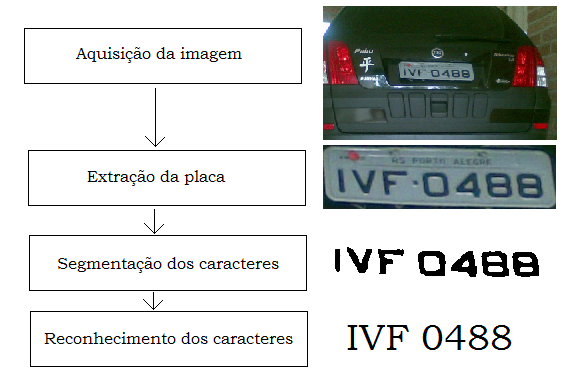
\includegraphics[width=88mm]{processo.png}
	\caption{Quatro estágios do reconhecimento de placa}
	\label{fig:processo}
\end{figure}

\section{Placa de Transito Brasileira}
\label{sec:placabr}

Segundo o código de transito brasileiro~\cite{brasil1997lei}, todos os veículos
são identificados por meio de placas, dianteira e traseira. Elas são
identificadas por uma tarja na parte superior contendo a sigla do estado e o
nome do município, e pelo código de identificação único, composto por três
letras, seguidas por quatro dígitos, separados por um hífen.

Veículos particulares, de aluguel, oficial, de experiência, de aprendizagem e de
fabricante têm suas dimensões de \emph{130mmx400mm} e altura dos caracteres de 63mm(figura~\ref{fig:placa_carro}).
Caso a placa não caiba no receptáculo ela pode ser reduzida em até 15\%. As
placas de motocicleta, motoneta, ciclomotor e triciclos autorizados tem
dimensões de \emph{136mmx187mm} e altura de caracteres de 42mm(figura~\ref{fig:placa_moto}).

\begin{figure}[H]
	\centering
	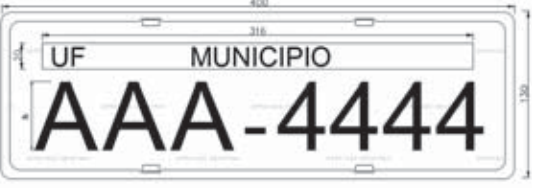
\includegraphics[width=88mm]{placa_carro.png}
	\caption{Placa de um carro}
	\label{fig:placa_carro}
\end{figure}

\begin{figure}[H]
	\centering
	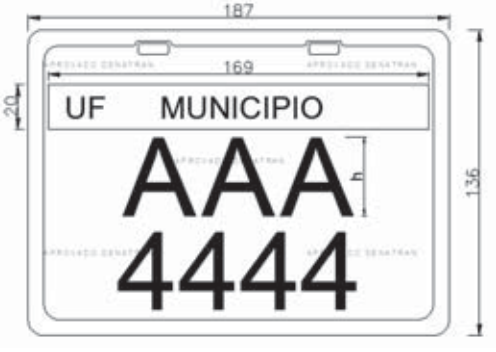
\includegraphics[width=88mm]{placa_moto.png}
	\caption{Placa de uma moto}
	\label{fig:placa_moto}
\end{figure}

A tipologia dos caracteres das placas utiliza a fonte
\emph{Mandatory}~\ref{fig:tipografia}, e as placas de categorias diferentes de veículos
são diferenciadas pelas suas cores.

\begin{figure}[H]
	\centering
	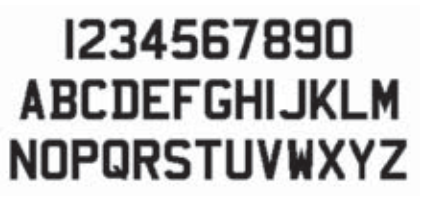
\includegraphics[width=88mm]{fonte.png}
	\caption{Tipografia das placas}
	\label{fig:tipografia}
\end{figure}

\section{Aquisição das imagens}
\label{sec:aquisicao}

O primeiro passo para o reconhecimento de uma placa é a extração das imagens. Diversos fatores
externos podem afetar o reconhecimento da placa, como a iluminação, a distância
e o ângulo da imagem. A influência desses fatores pode ser minimizada
utilizando-se de imagens de qualidade.

A aquisição das imagens será feita utilizando o módulo de câmera do
\emph{Raspberry Pi}. É uma câmera de 5 \emph{megapixels} capaz de gravar vídeos
em 1080p. Uma das vantagens de utilizar essa combinação do \emph{Raspberry Pi} e
seu módulo de câmera é a sua portabilidade. Por serem pequenos e leves, caso a
câmera tenha dificuldade em capturar imagens de qualidade para o reconhecimento
das placas, é possível movê-los e colocá-los em posições privilegiadas para
otimizar o processo.

\section{Extração da placa}
\label{sec:extracao}

A fase de extração é a fase mais importante em um sistema de reconhecimento de
placas, porque todas as outras fases dependem da exata extração da área da
placa. Essa extração é difícil pois influencia na precisão do sistema como um
todo~\cite{kaur2014efficient}. Muitas dificuldades podem ocorrer durante a fase
de extração pelos seguintes motivos:

\begin{itemize}
	\item A eficiência da extração é afetada pela complexidade da cena.
	\item Diferentes veículos possuem suas placas em diferentes posições.
	\item Pode ocorrer ruído durante a captura da câmera.
	\item Condições do tempo pode influenciar no ruído.
	\item Hora do dia afeta na luminosidade e resulta em erros de contraste.
	\item Outros caracteres, quadros e parafusos podem introduzir confusão.
	\item Mal posicionamento da câmera, ou placa, pode resultar em distorção que afeta na eficiência.
	\item Luminosidade baixa, ou desigual, imagem desfocada, baixa resolução, reflexão, sombra afetam a eficiência da extração.
\end{itemize}

O método implementado é baseado em Kaur~\cite{kaur2014efficient} e segue o seguinte fluxograma:

\begin{enumerate}
	\item Conversão de RGB para escala de tons de cinza
	\item Remoção de ruído por filtro bilateral
	\item Aumento de contraste usando equalização de histograma adaptativo
	\item Binarização da Imagem
	\item Detecção de borda pelo operador \emph{Sobel}
	\item Detecção de Área de Placa Candidata por Operações Morfológicas de Abertura e Fechamento
	\item Extração da área da placa real
    \item Aprimoramento da região extraída
\end{enumerate}

\subsection{Conversão de RGB para escala de tons de cinza}

A imagem capturada está no formato RGB\@. O primeiro passo do pré-processamento é
converter essa imagem para a escala de tons de cinza. O objetivo dessa conversão é reduzir
o número de cores. Os componentes R, G e B são separados do valor de cor de 24
bits de cada pixel (i,j), e um valor de 8 bits em cinza é calculado.

\begin{figure}[H]
	\centering
	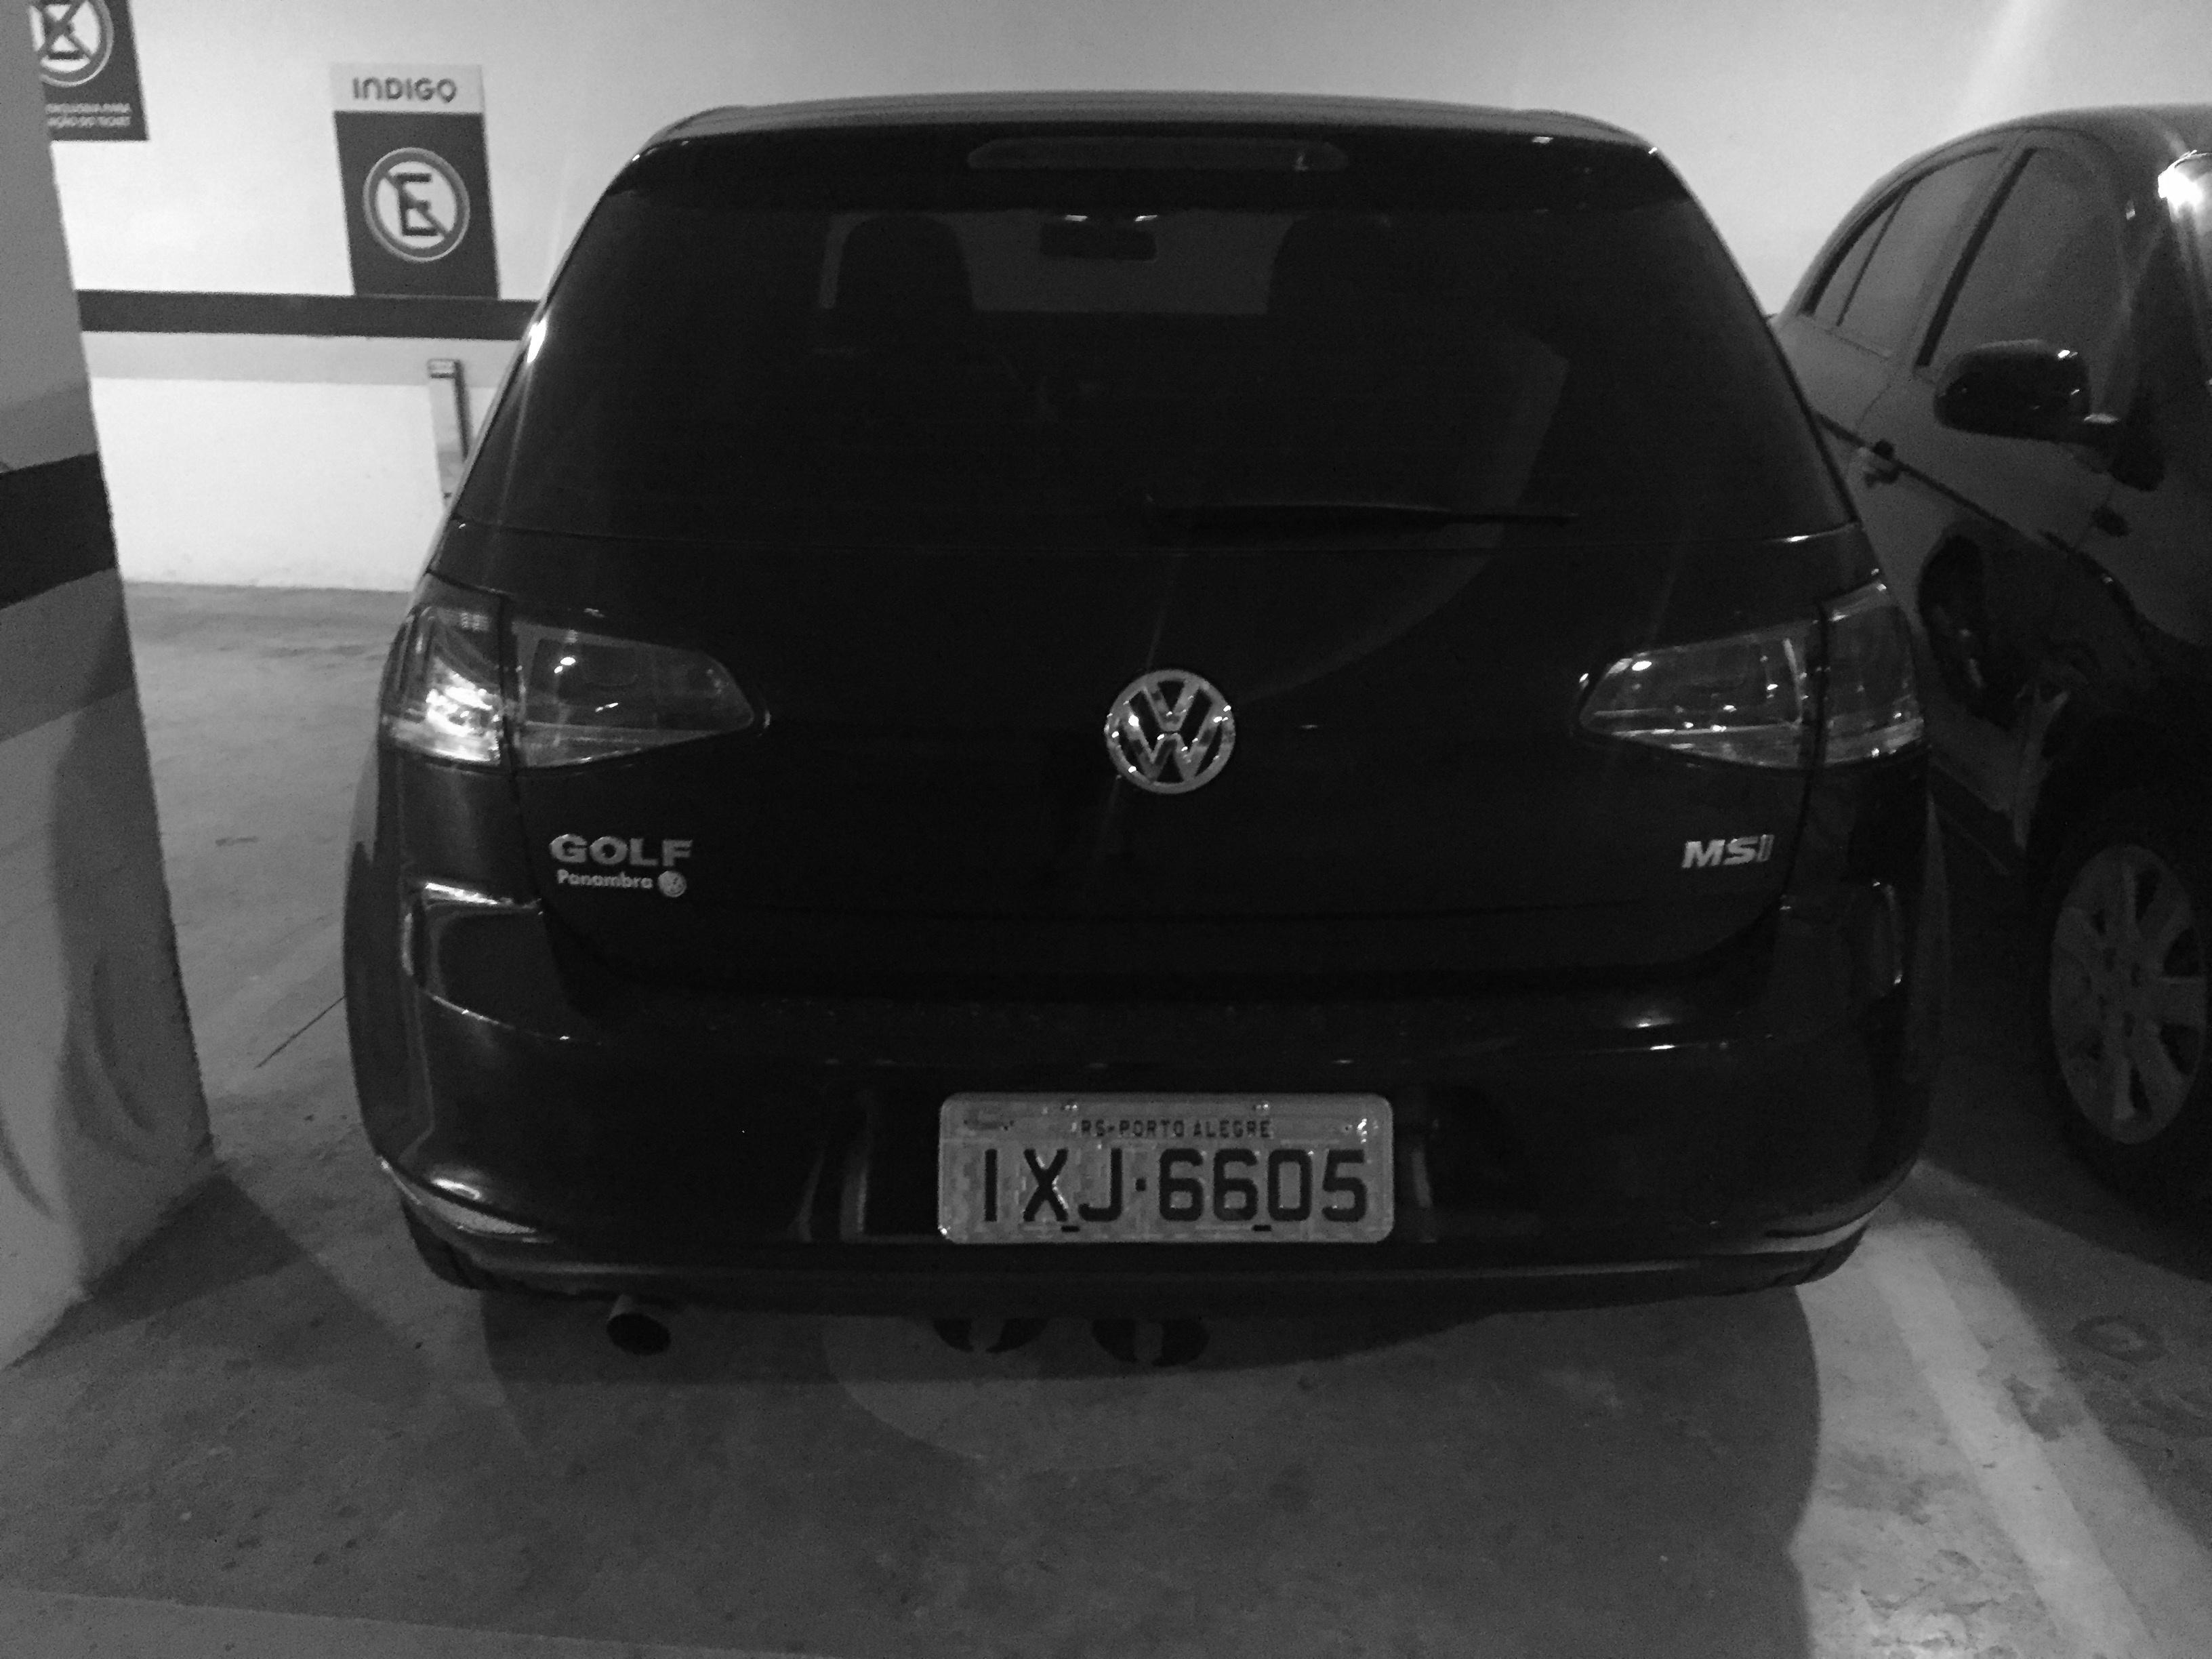
\includegraphics[width=88mm]{1grayscale.jpg}
	\caption{Imagem em escala de tons de cinza}
Fonte: Imagem processada pelo algoritmo
	\label{fig:ext_gray_scale}
\end{figure}

\subsection{Remoção de ruído por filtro bilateral}

O filtro bilateral é um filtro não linear, que preserva as arestas e reduz ruído.
Ele funciona substituindo o valor de intensidade de cada \emph{pixel} em uma imagem
por uma média ponderada dos valores de intensidade dos \emph{pixels} próximos.
O objetivo básico da filtragem é remover ruído e distorção da imagem. O ruído
pode ocorrer durante a captura pela câmera ou pelas condições do tempo. No
método que Kaur~\cite{kaur2014efficient} propõe, filtro bilateral iterativo é
utilizado para remover ruído. Ele é não linear, provê mecanismo para remoção de
ruído enquanto preserva bordas mais efetivamente que o filtro mediano. O filtro
mediano funciona substituindo o valor de cada \emph{pixel} pela mediana dos \emph{pixels}
vizinhos.

\begin{figure}[H]
	\centering
	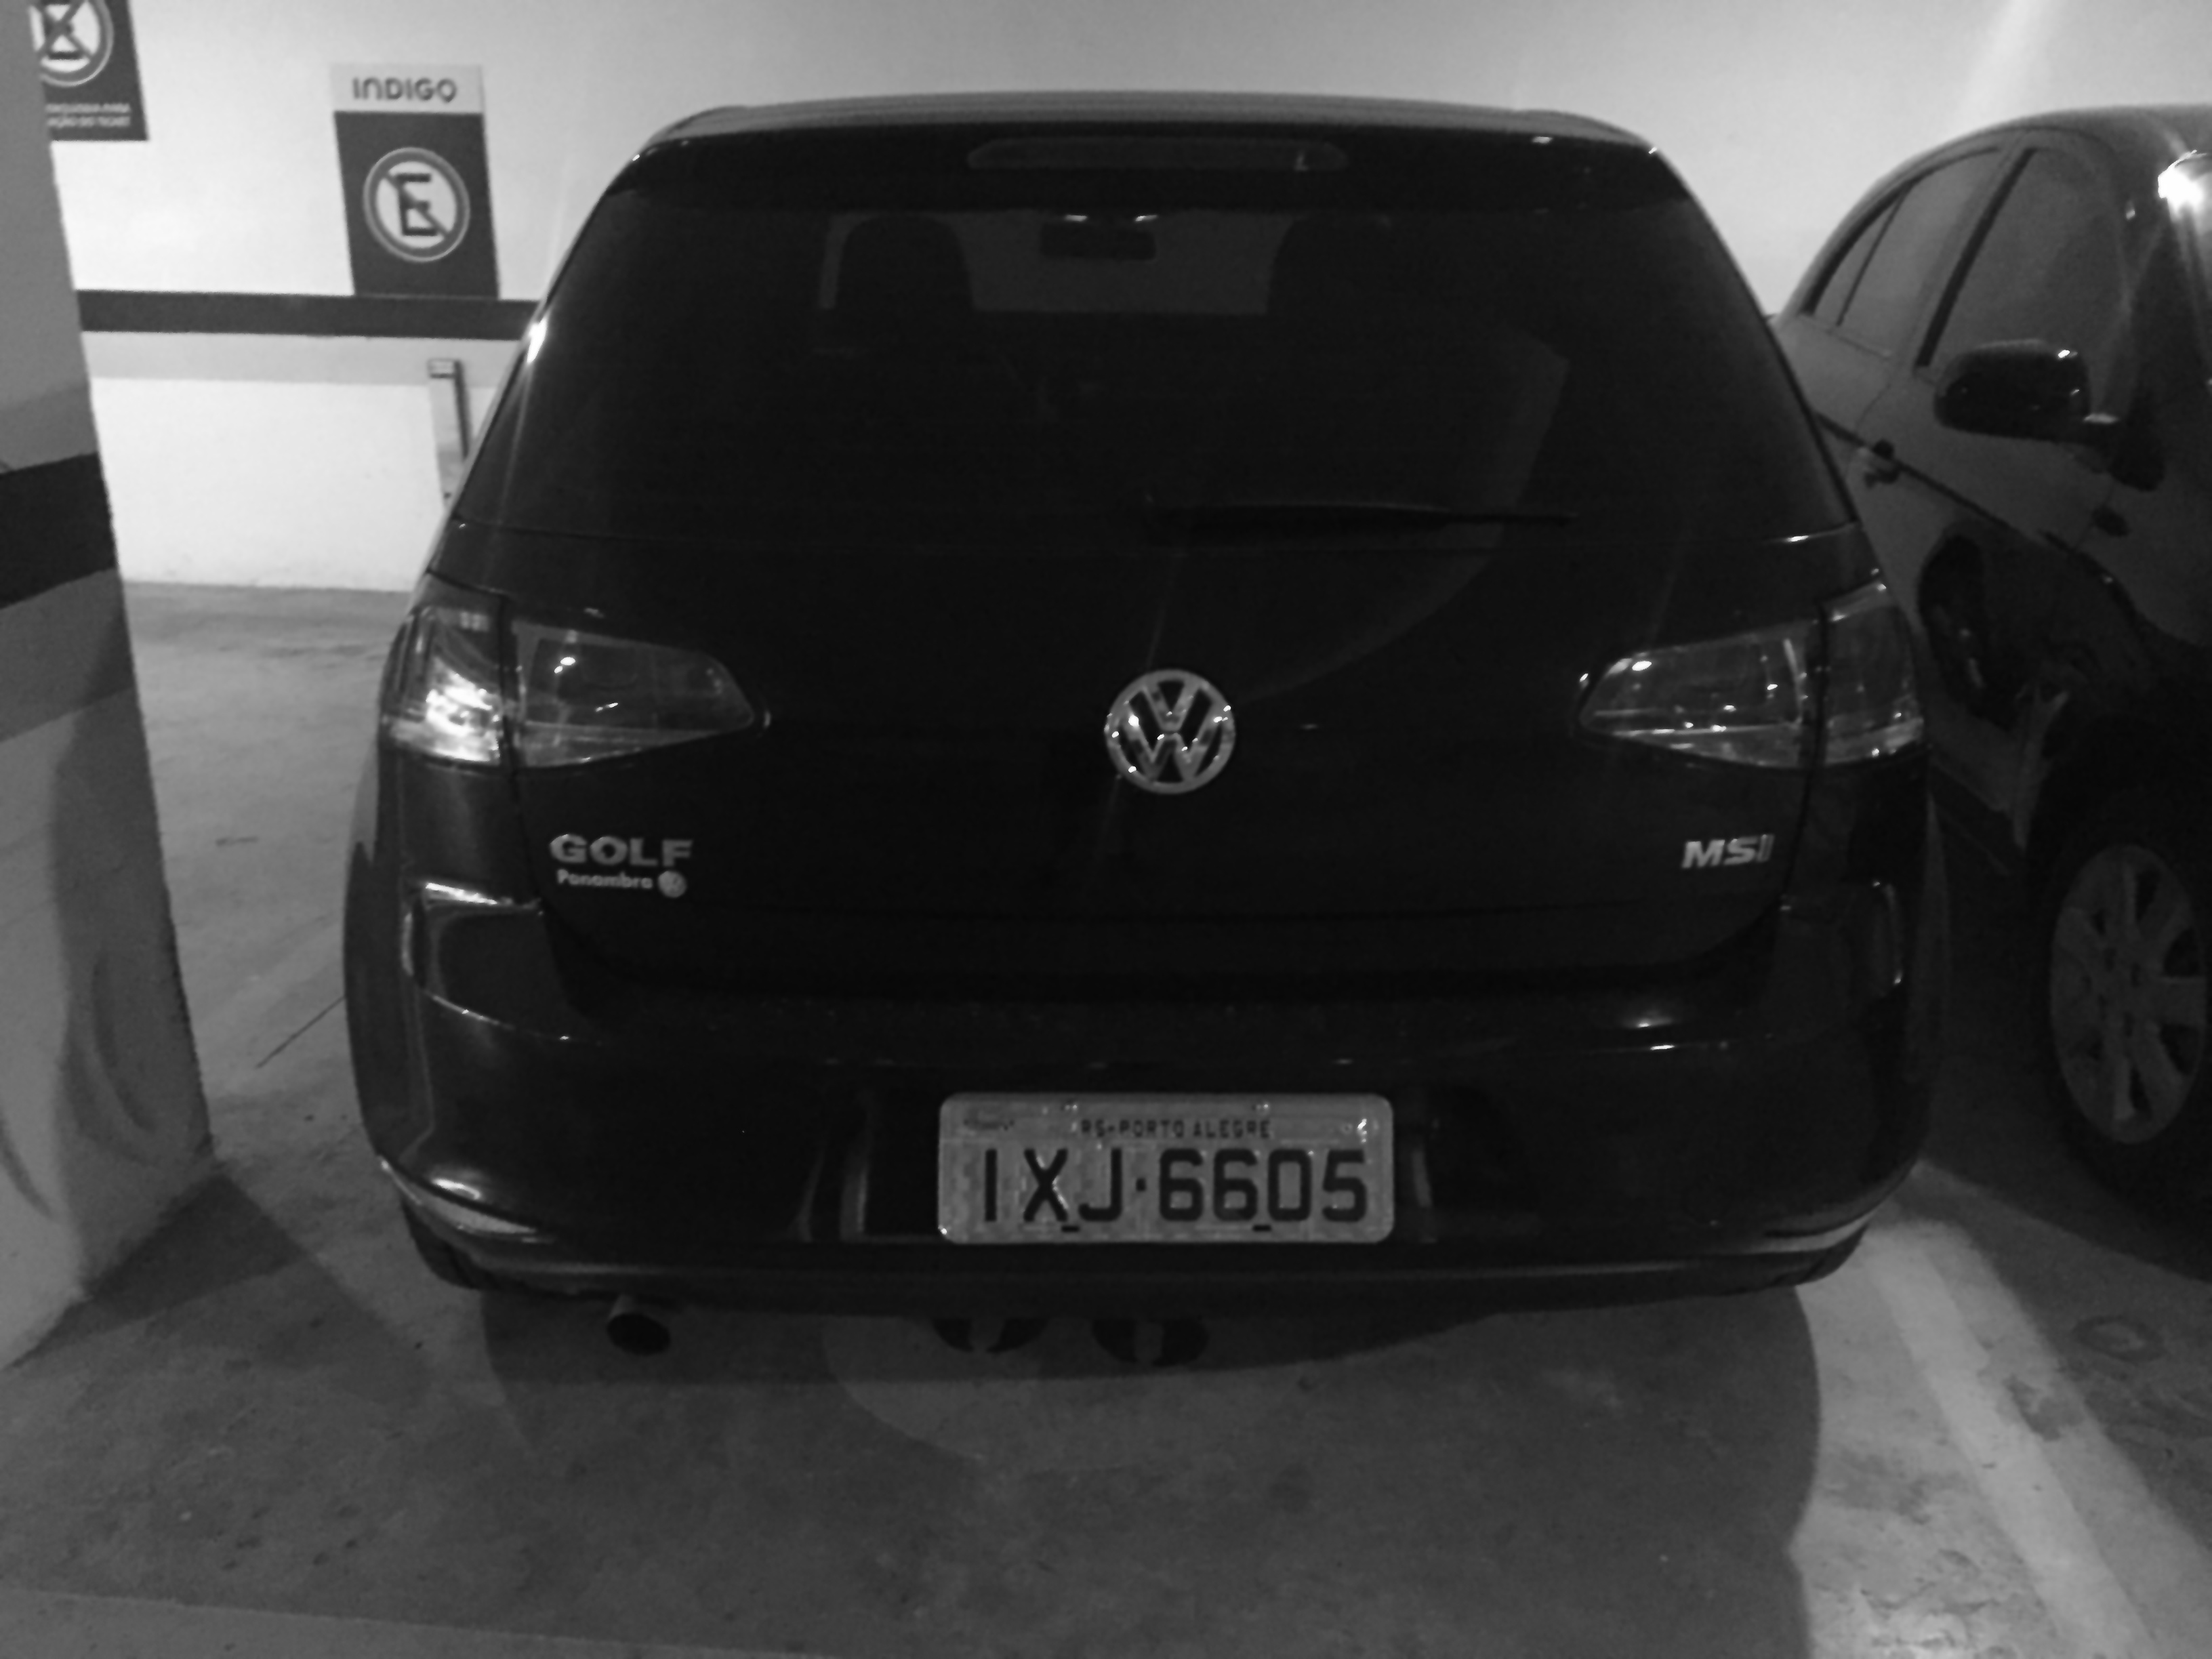
\includegraphics[width=88mm]{2bilateral.jpg}
	\caption{Aplicação de filtro bilateral em uma imagem em escala de tons de cinza}
Fonte: Imagem processada pelo algoritmo
	\label{fig:ext_filter_in_gray_scale}
\end{figure}

\subsubsection{Aumento de contraste usando equalização de histograma adaptativo}

Contraste é definido como a diferença entre o nível mais baixo e alto de
intensidade. Equalização de histograma é o método para distribuir de forma mais
efetiva o histograma de \emph{pixels}. Equalização de histograma adaptativo
mostra melhor contraste em relação a equalização de histograma.

\begin{figure}[H]
	\centering
	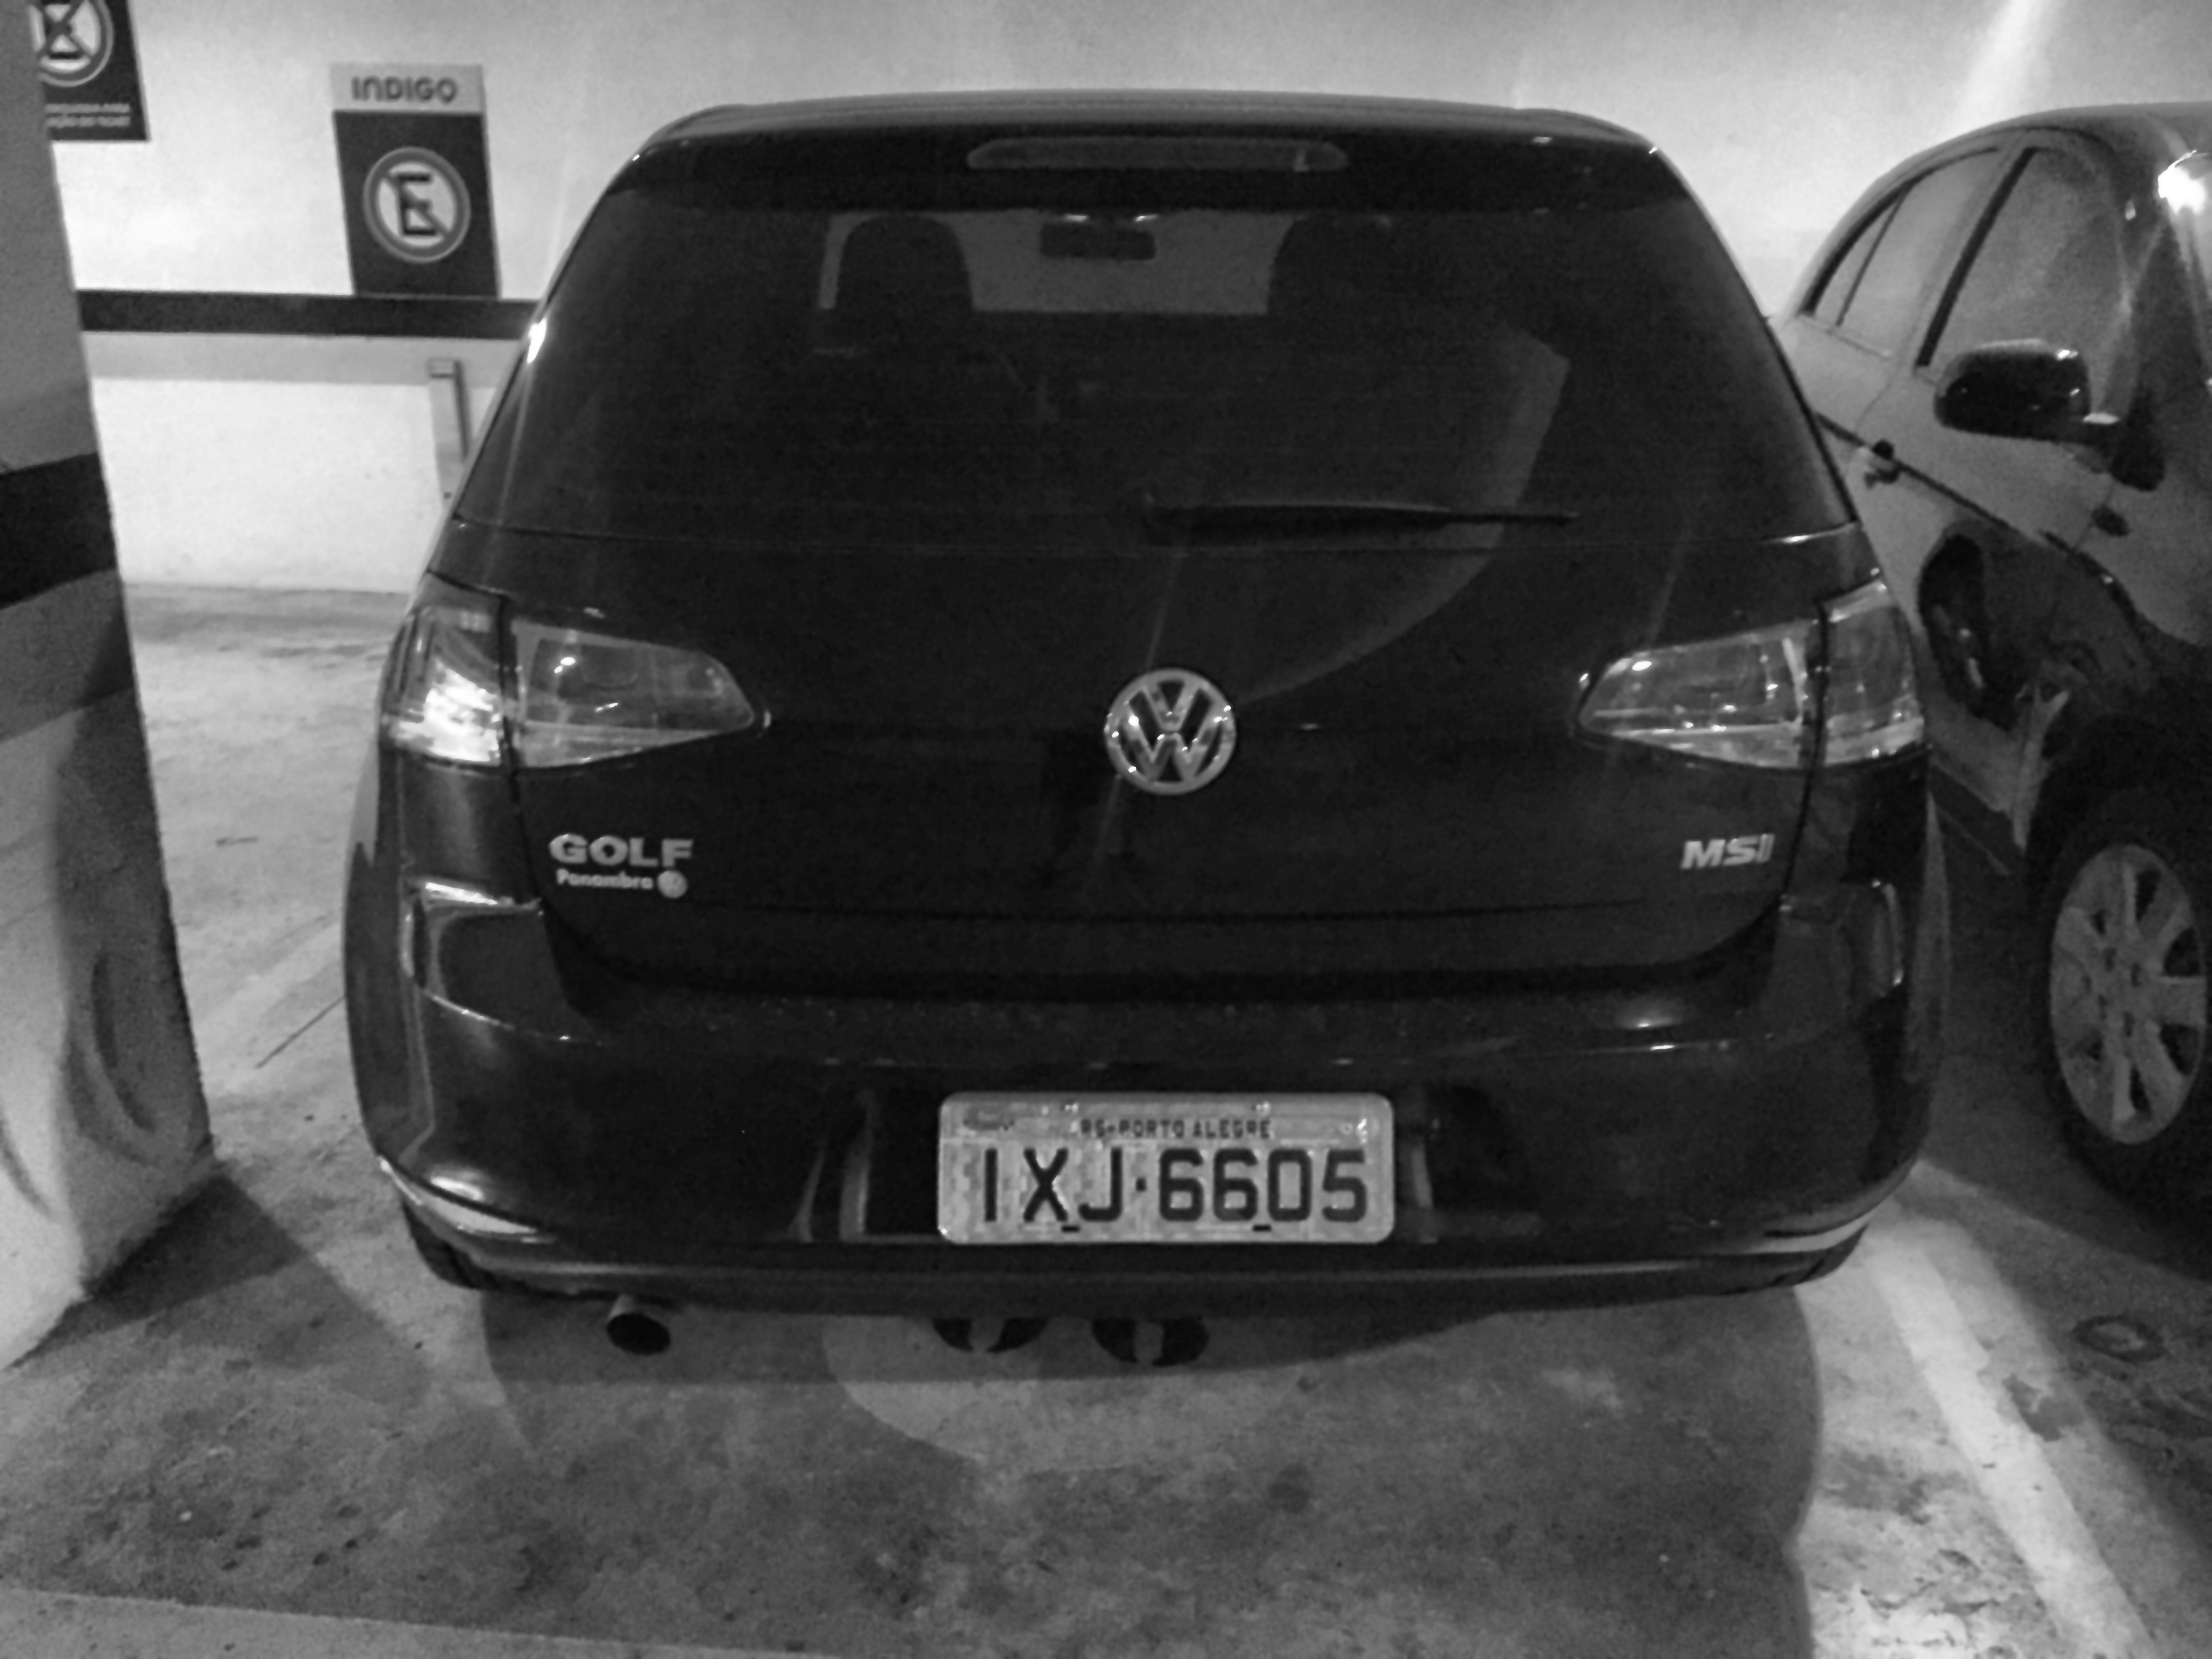
\includegraphics[width=88mm]{3histogram_eq.jpg}
	\caption{Aumento de contraste usando equalização de histograma adaptativo}
Fonte: Imagem processada pelo algoritmo
	\label{fig:ext_contrast_adaptive_histogram}
\end{figure}

\subsection{Binarização da Imagem}

Nesta operação a imagem de escala de cinza subtraída é convertida em imagem
binária. Em primeiro lugar, o nível de limiar é calculado pelo método de \emph{Otsu}.
O algoritmo do método de \emph{Otsu} assume que  a imagem contém duas classes de pixels
seguindo um histograma bi-modal. Ele então calcula o limiar ótimo separando as
duas classes para que o seu espalhamento combinado seja mínimo.
Tendo o limiar calculado, a imagem de escala de cinza subtraída é convertida em
imagem em preto e branco.

\begin{figure}[H]
	\centering
	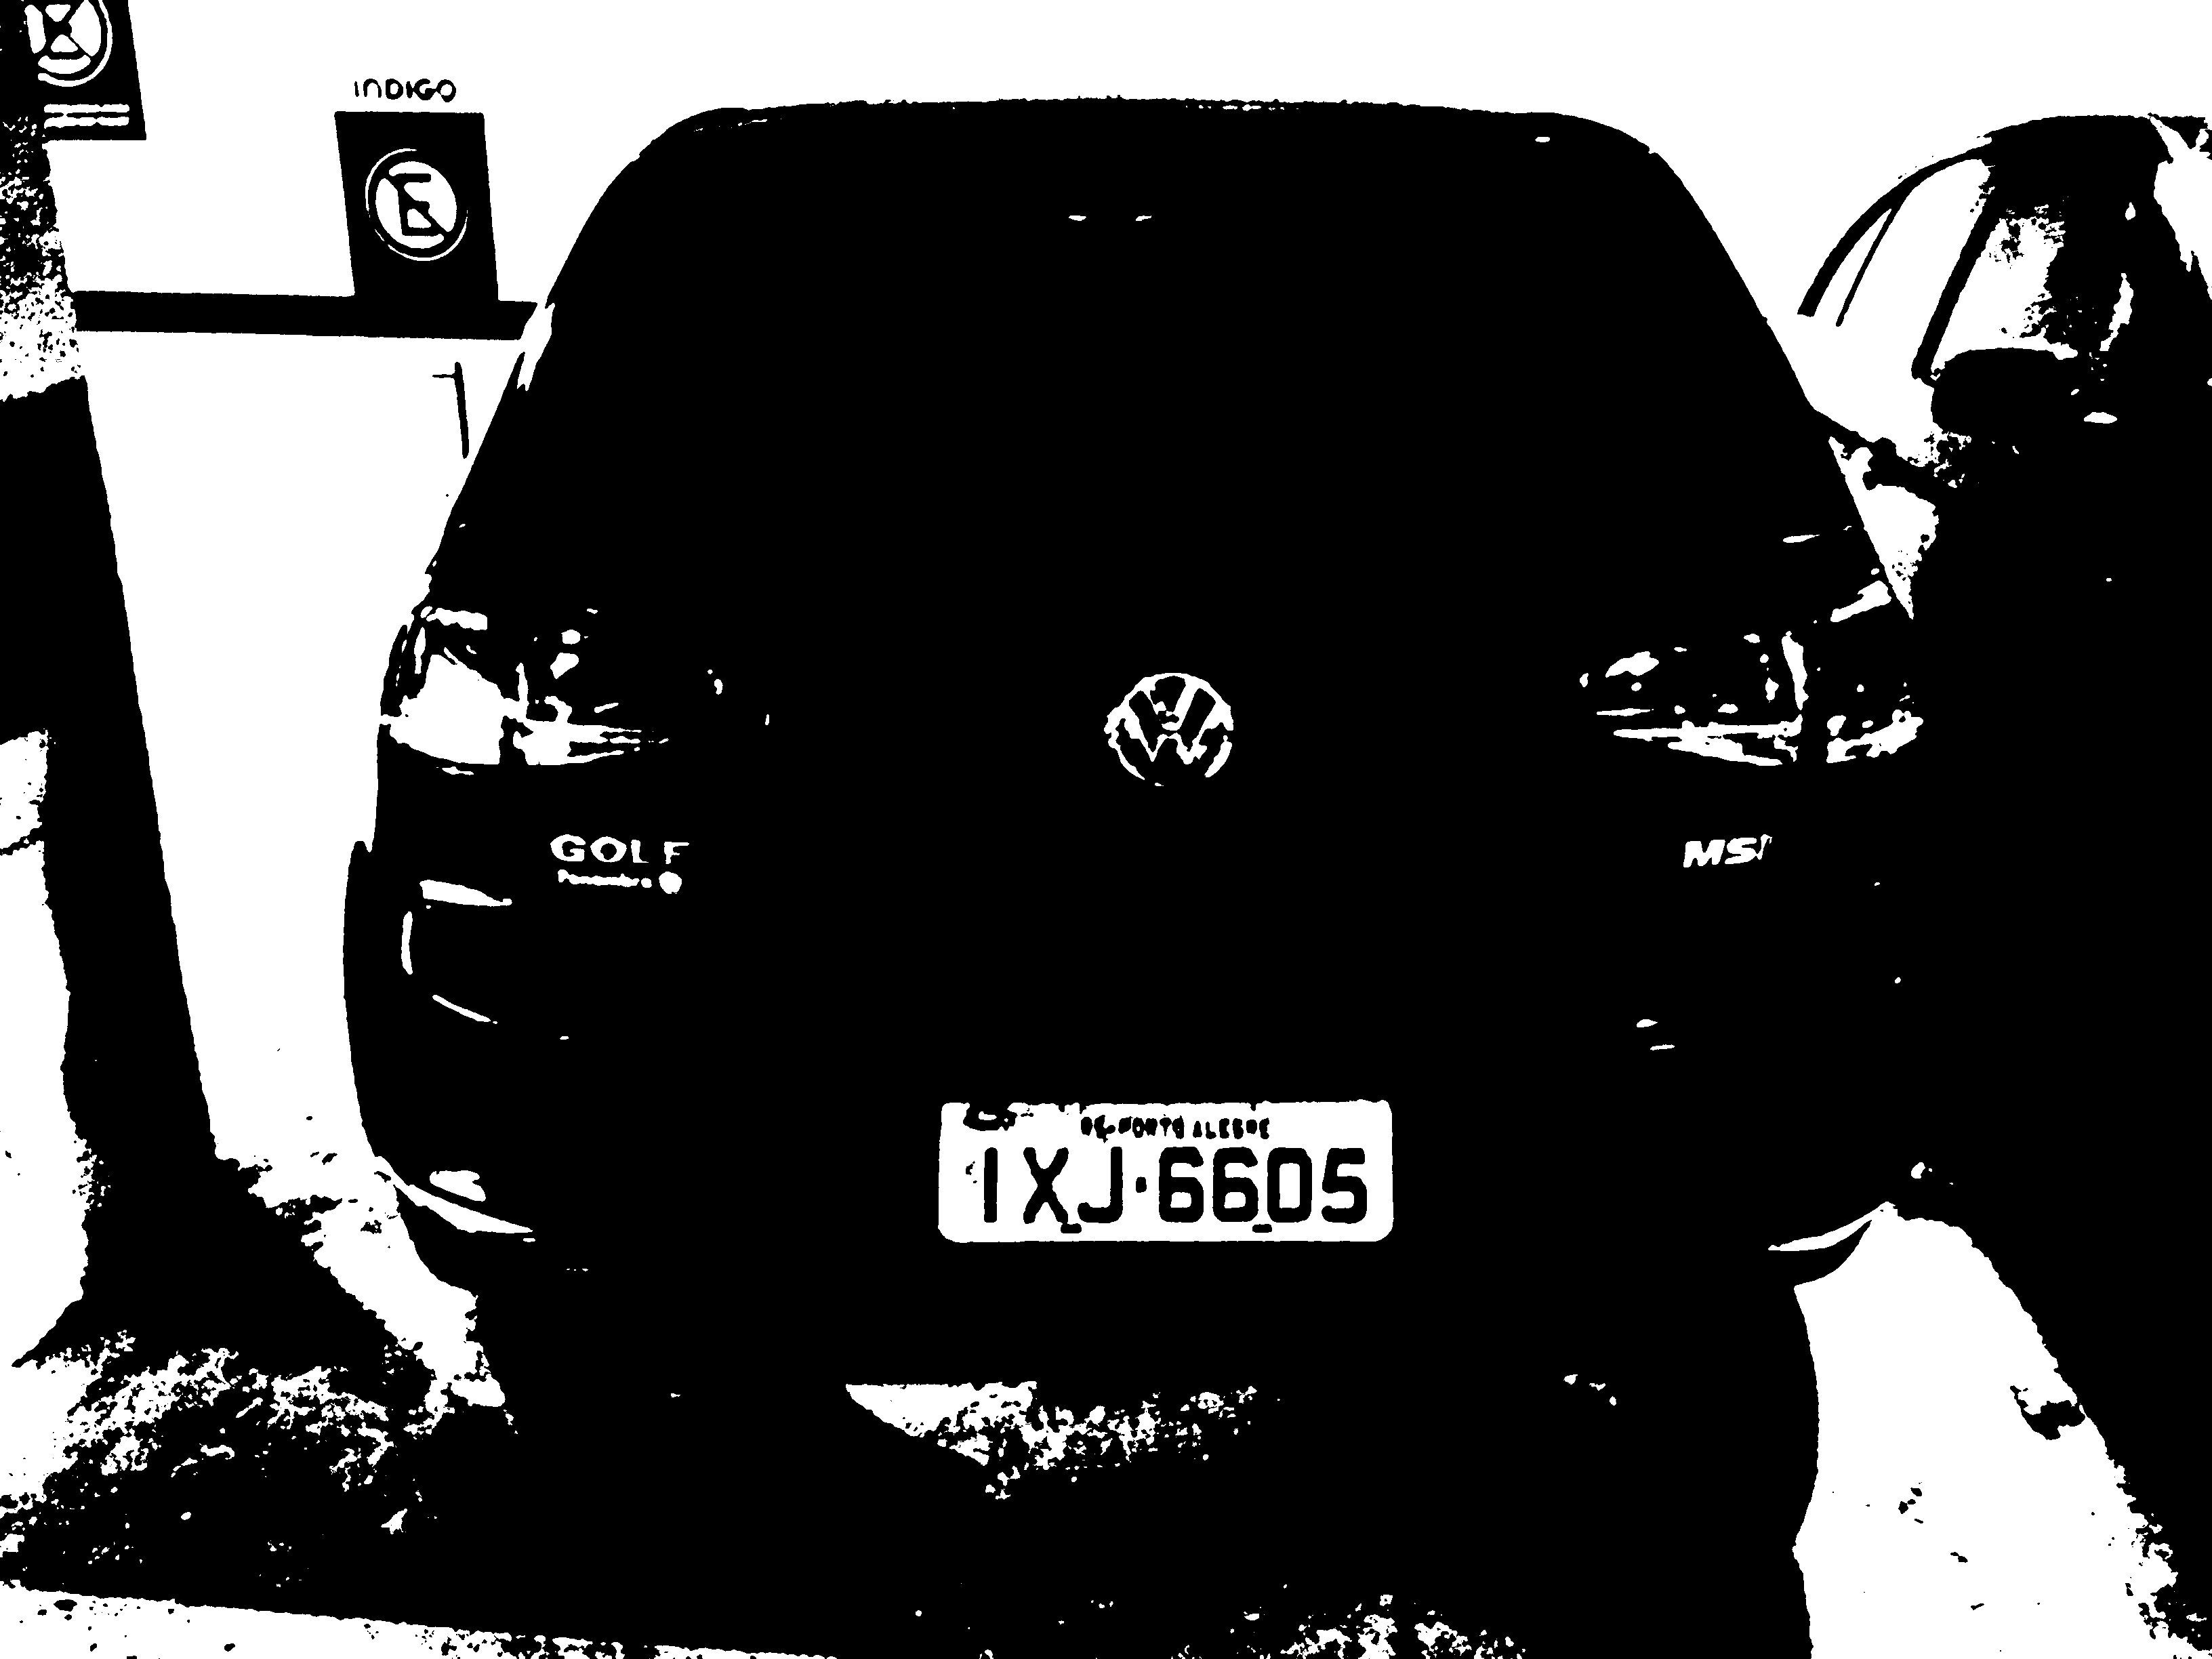
\includegraphics[width=88mm]{4binarized_image.jpg}
	\caption{Imagem Binarizada}
Fonte: Imagem processada pelo algoritmo
	\label{fig:ext_binarized_image}
\end{figure}

\subsection{Detecção de borda pelo operador Sobel}

A borda vertical é detectada pelo operador \emph{Sobel} e o resultado do operador \emph{Sobel}
ser aplicado à imagem binarizada é mostrado na figura~\ref{fig:ext_edge_detection_sobel}

\begin{figure}[H]
	\centering
	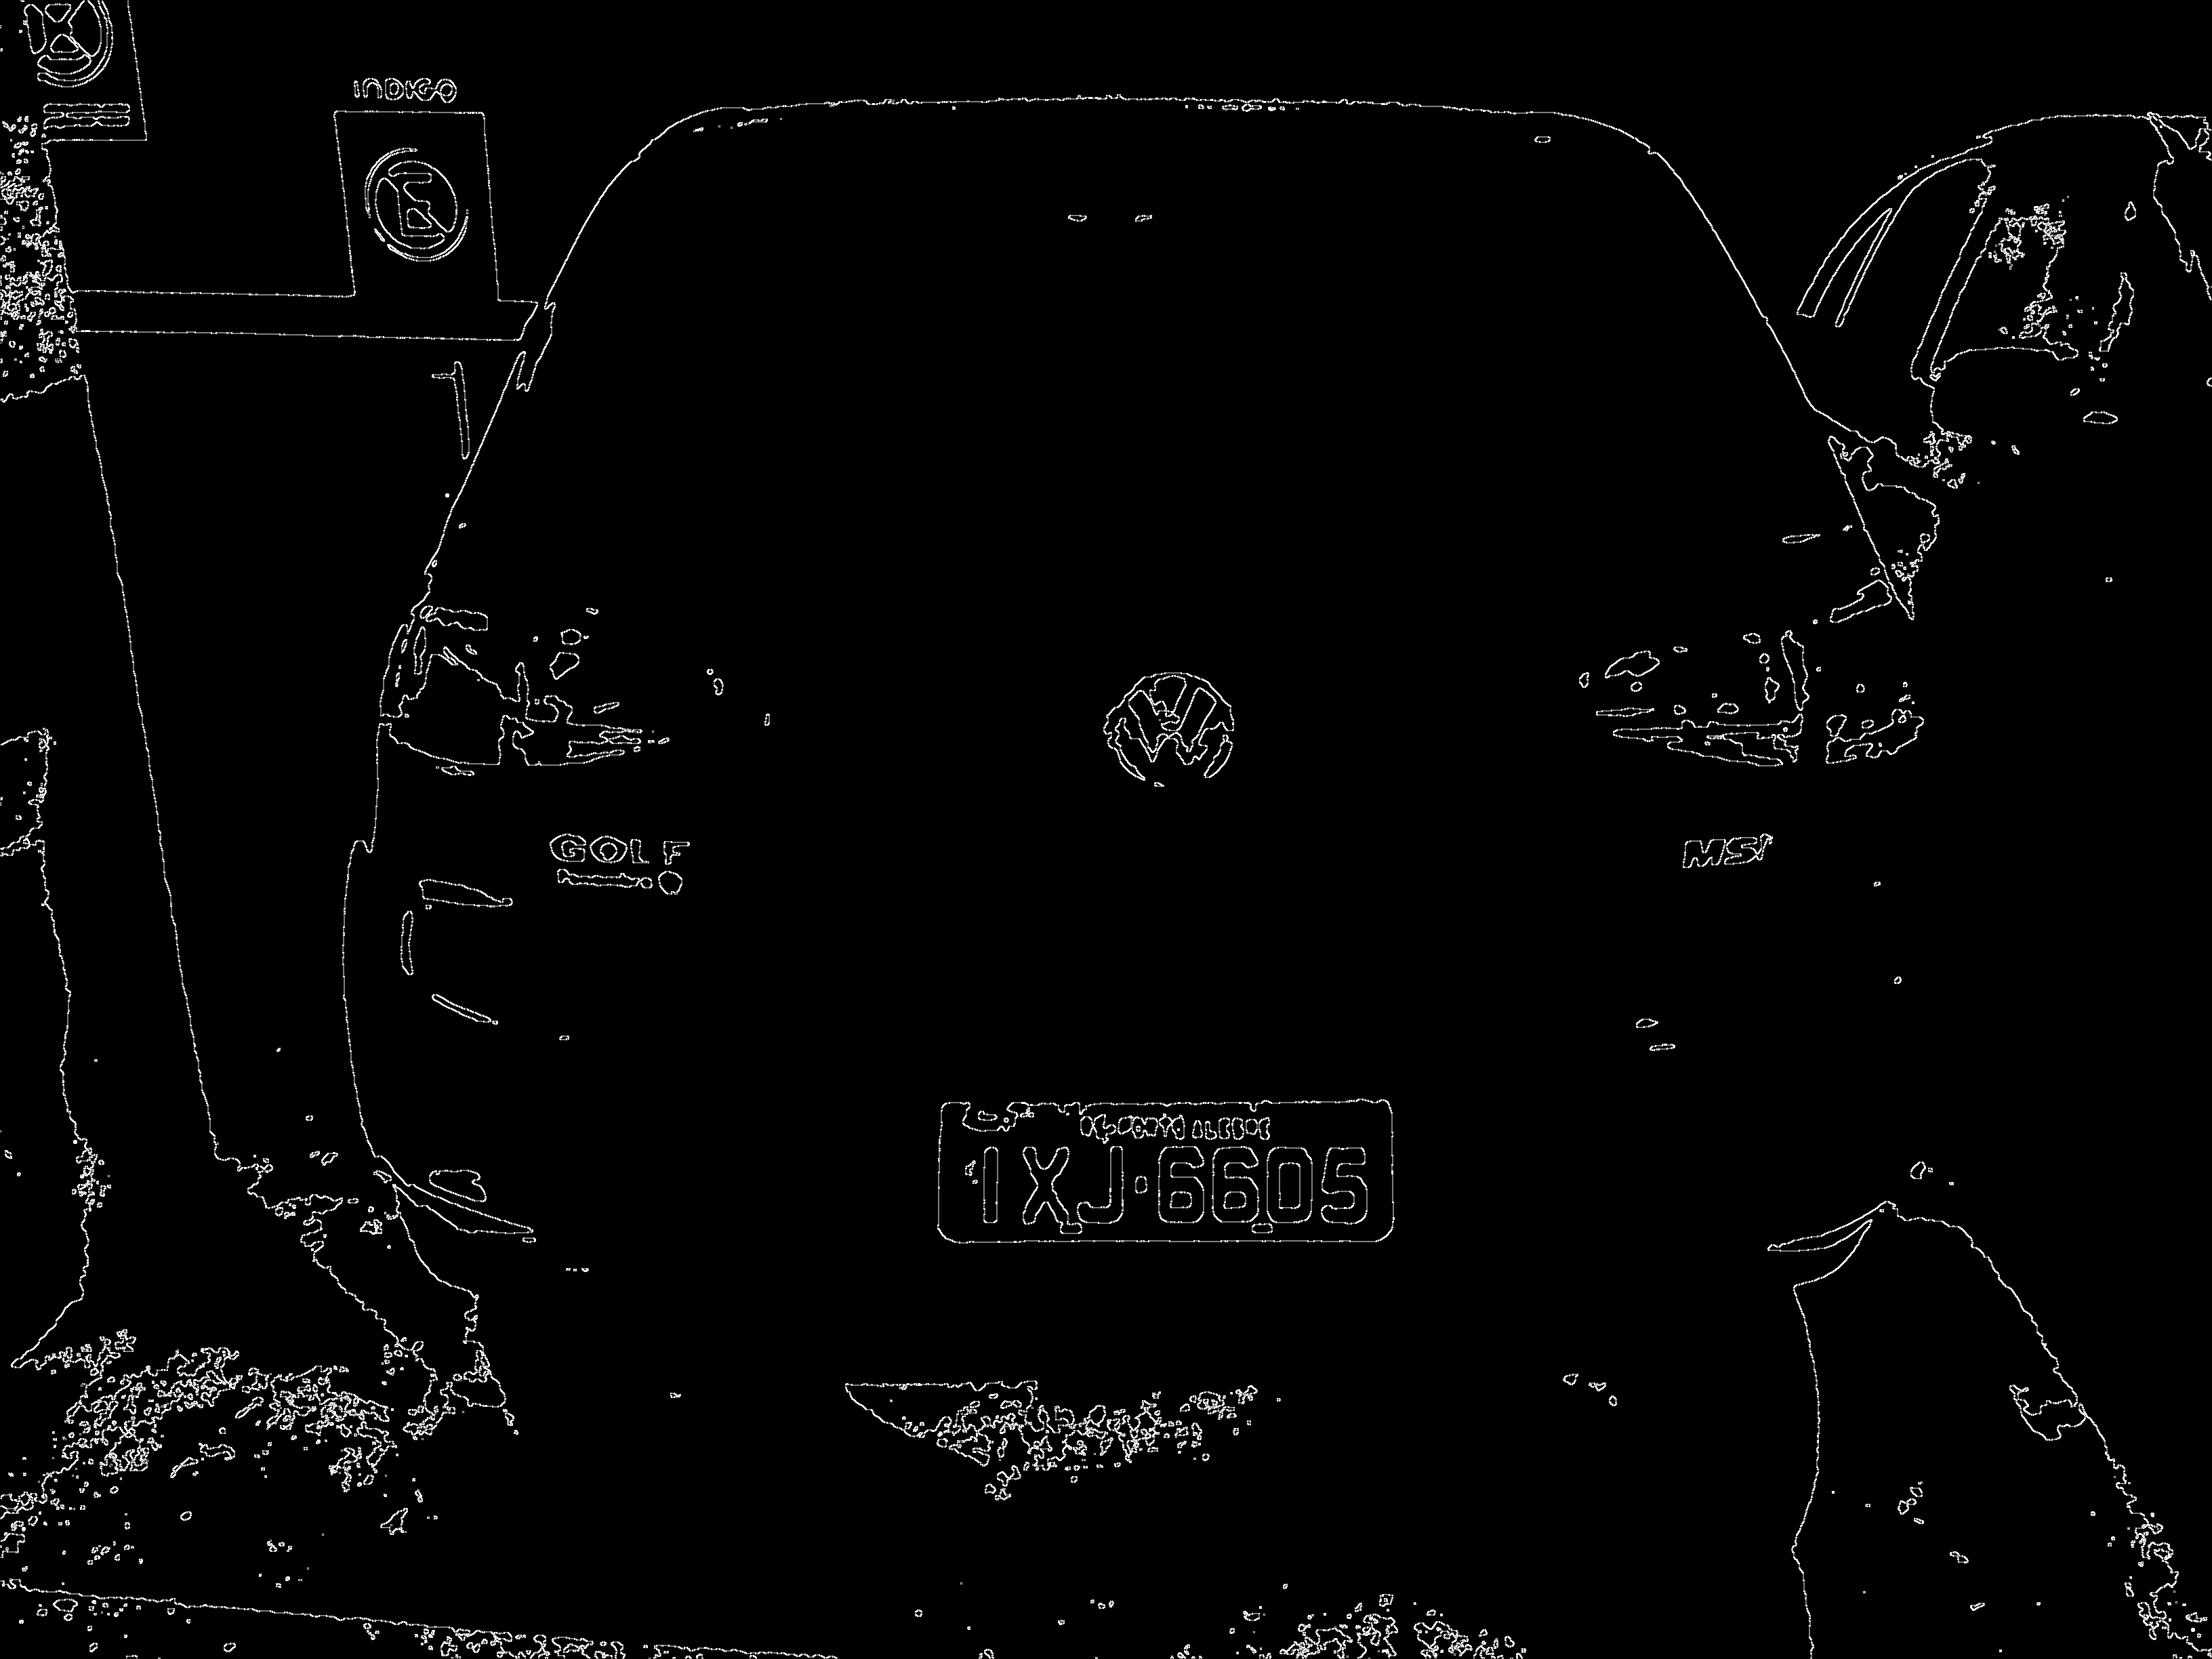
\includegraphics[width=88mm]{5sobel_image.jpg}
	\caption{Detecção de borda pelo operador Sobel}
Fonte: Imagem processada pelo algoritmo
	\label{fig:ext_edge_detection_sobel}
\end{figure}

\subsection{Detecção de Áreas de Placa Candidatas por Operações Morfológicas de Abertura e Fechamento}

Com as operações morfológicas, os objetos indesejados na imagem são removidos.
Para a detecção da área da placa, uma operação de dilatação é aplicada na imagem
e depois os buracos são fechados. Em seguida, operações de abertura morfológica
e erosão são usadas para a detecção exata da área da placa.

\begin{figure}[H]
	\centering
	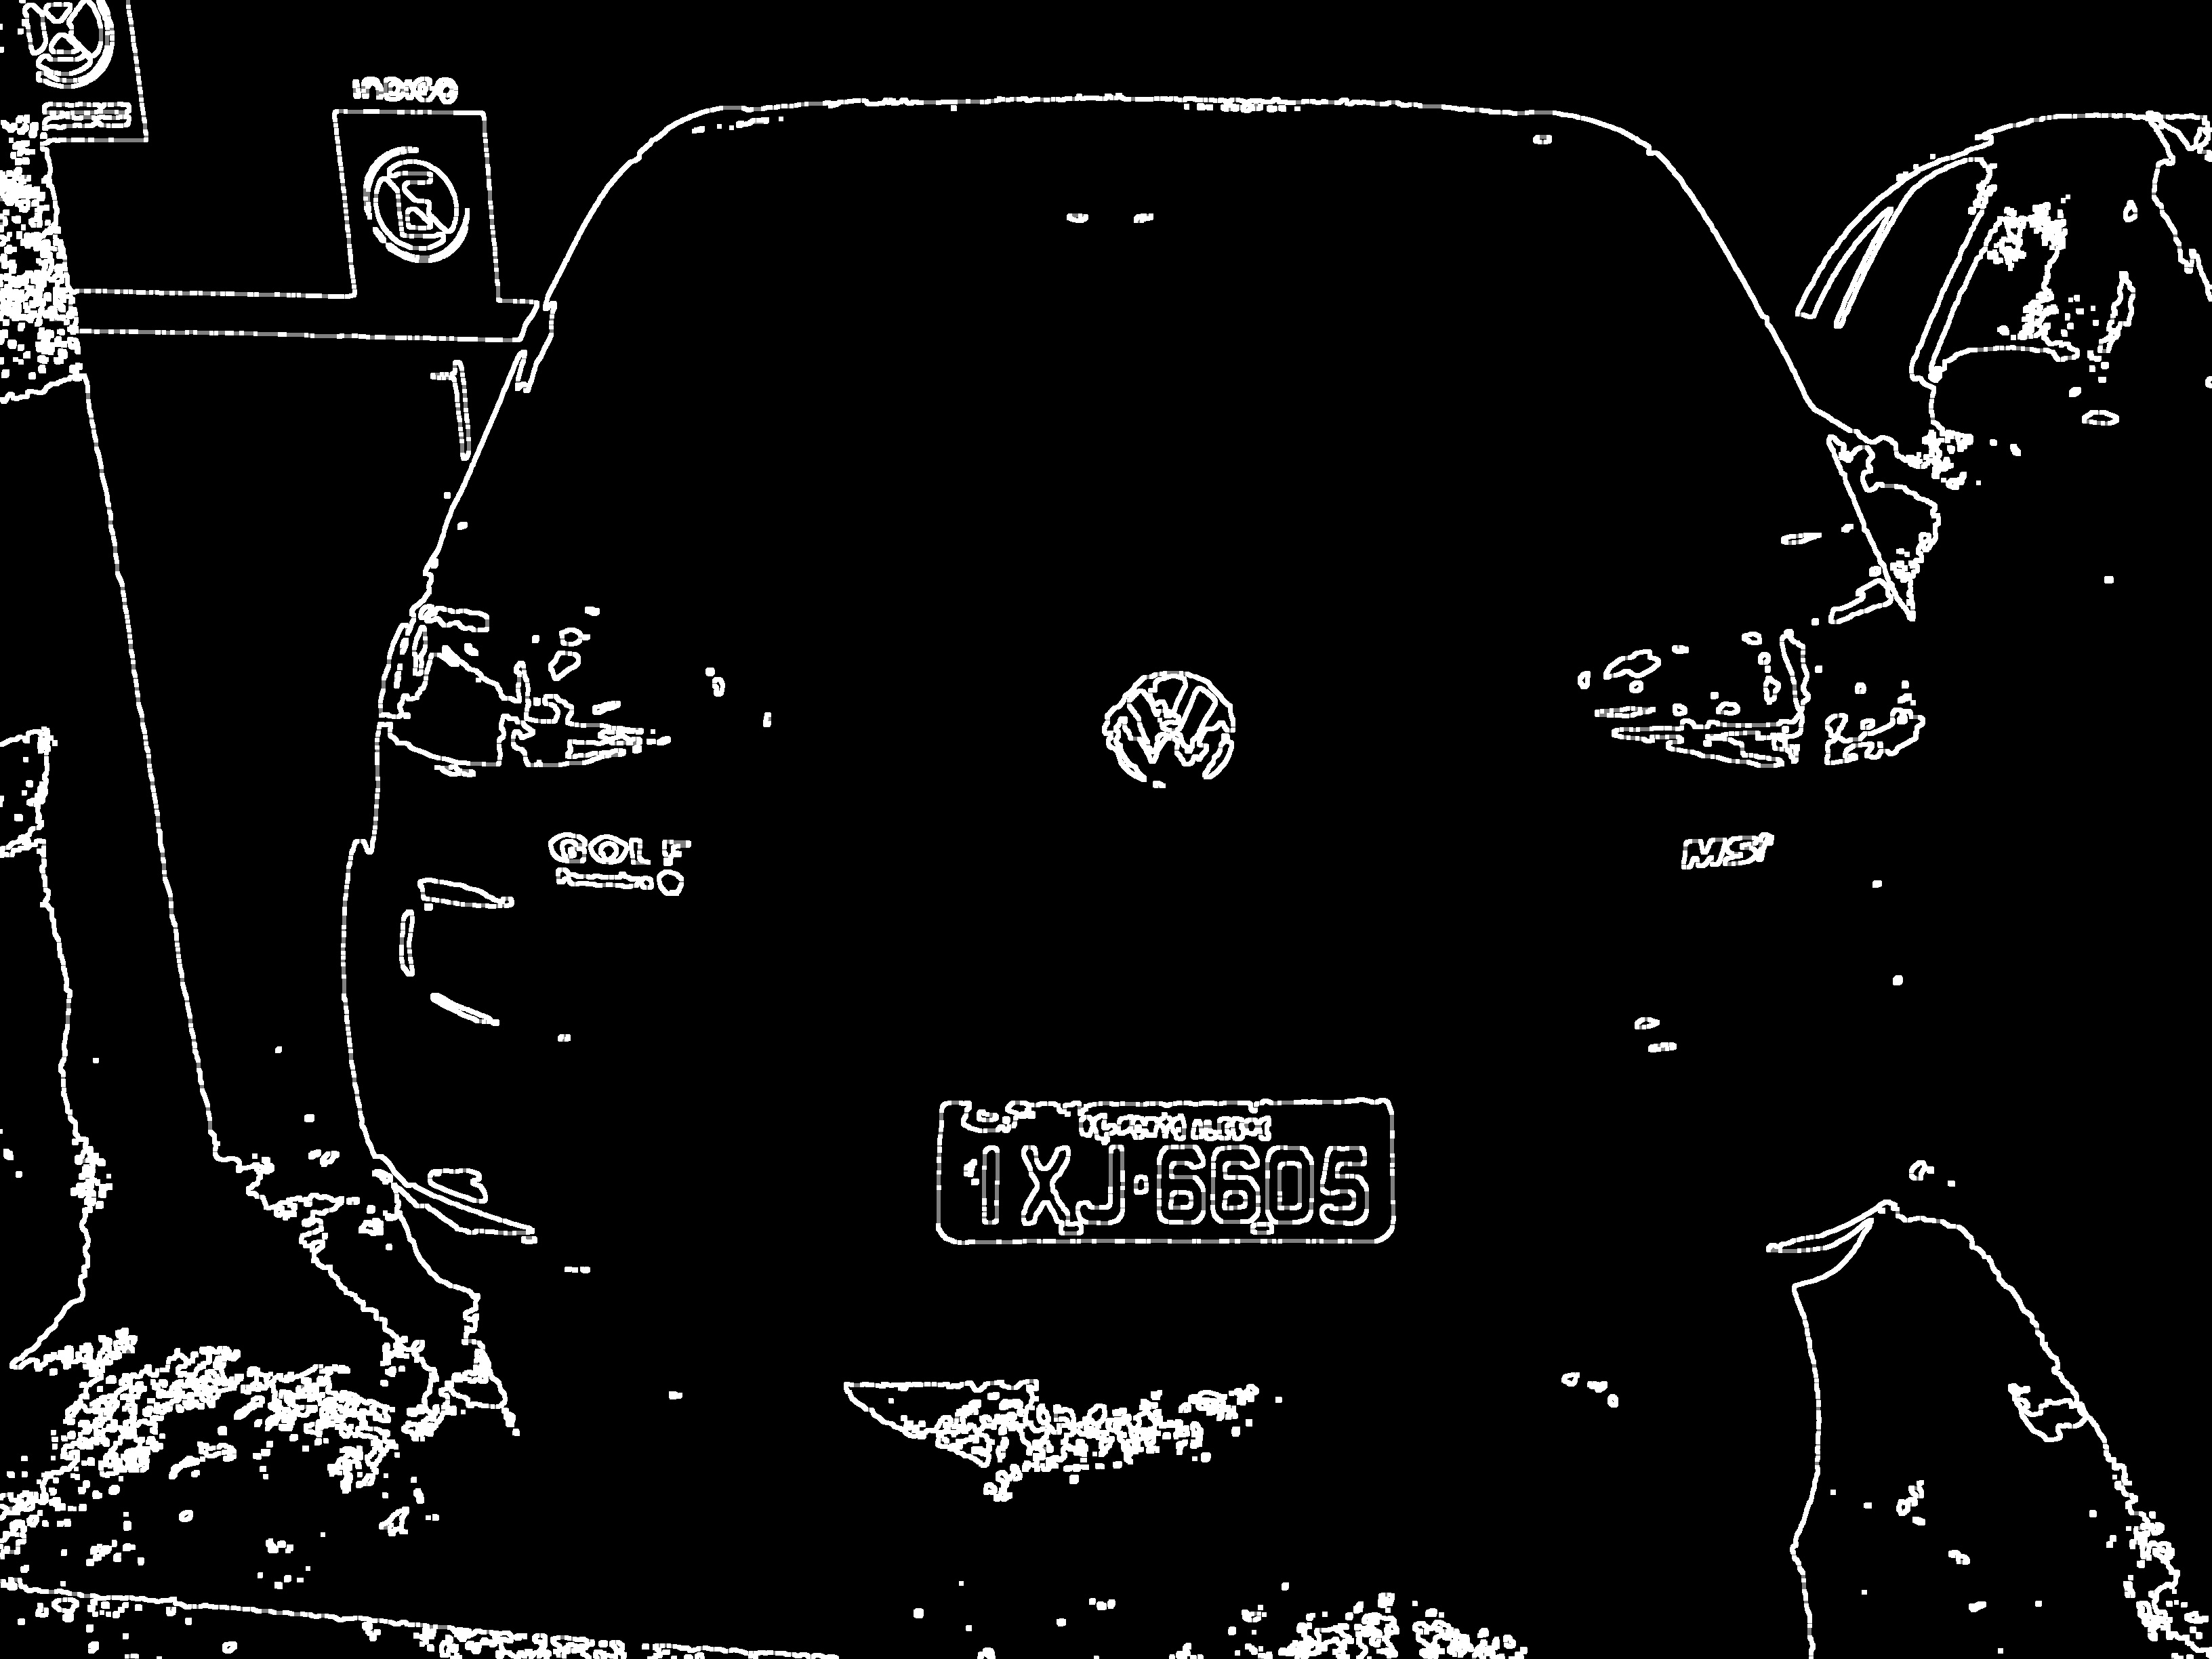
\includegraphics[width=88mm]{6dilated_image.jpg}
	\caption{Dilatação morfológica}
Fonte: Imagem processada pelo algoritmo
	\label{fig:ext_morphological_dilation}
\end{figure}

\begin{figure}[H]
	\centering
	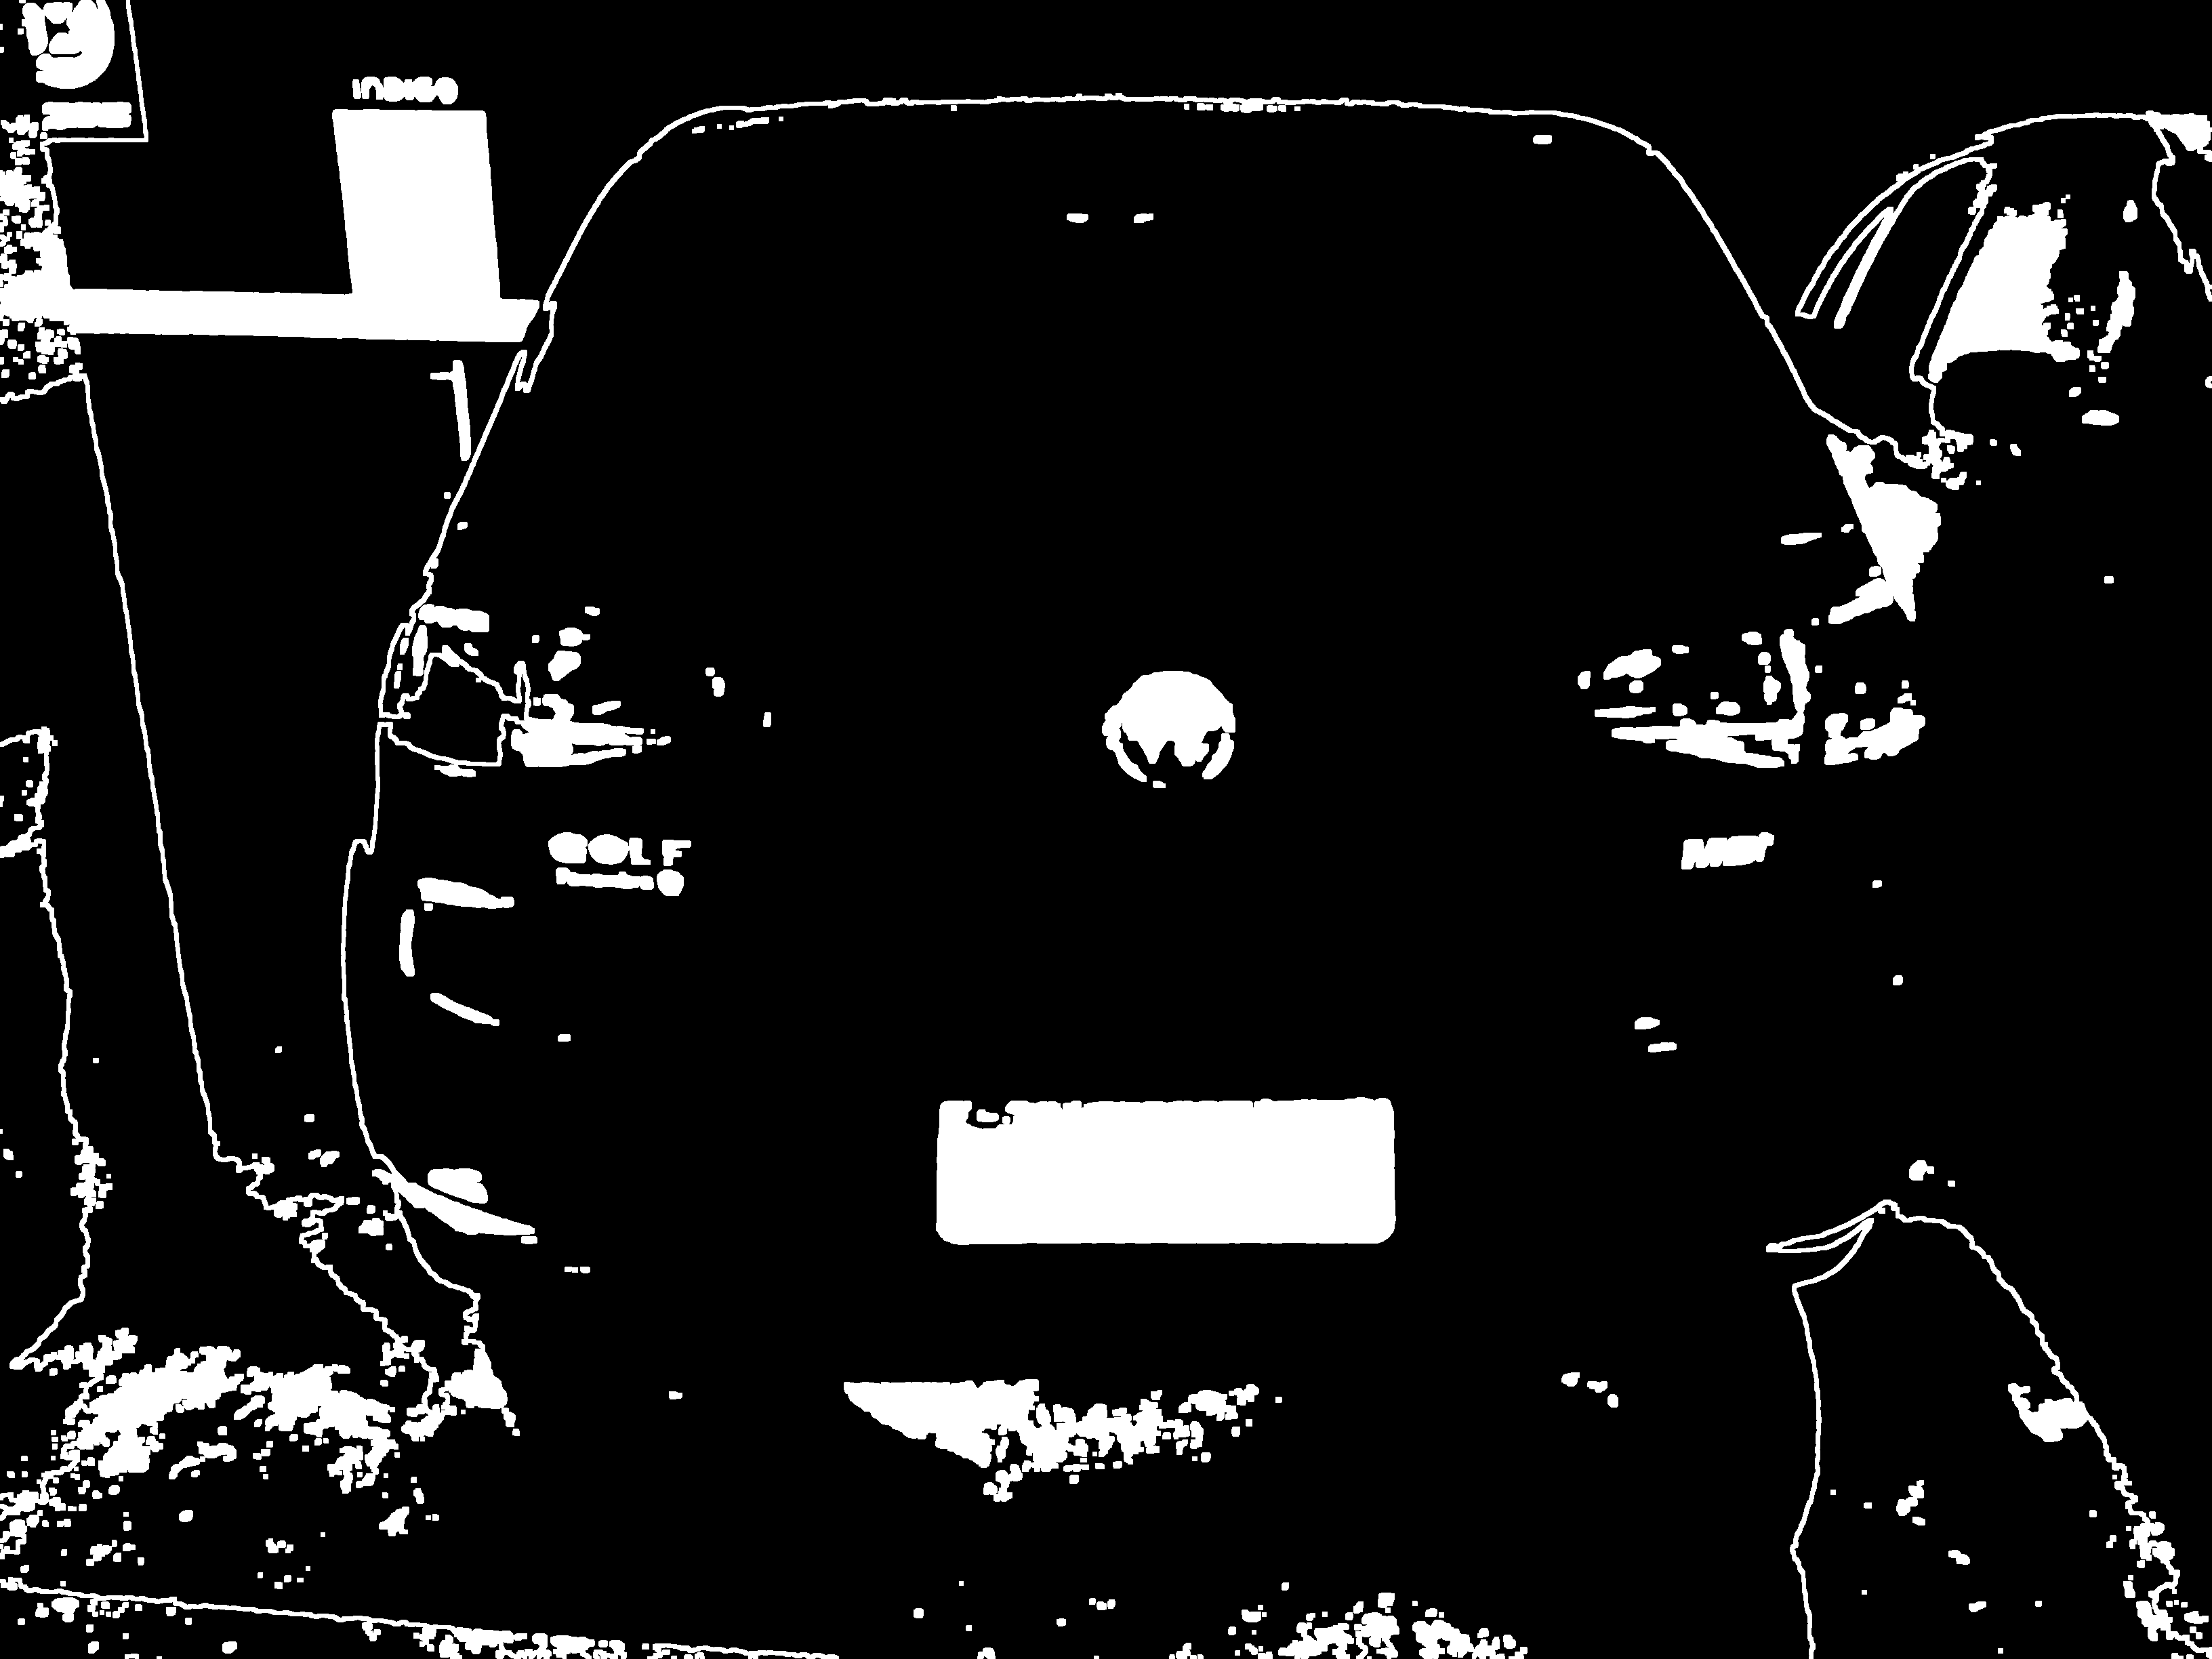
\includegraphics[width=88mm]{7filled_image.png}
	\caption{Após preenchimento dos buracos}
Fonte: Imagem processada pelo algoritmo
	\label{fig:ext_holes_filled}
\end{figure}

\begin{figure}[H]
	\centering
	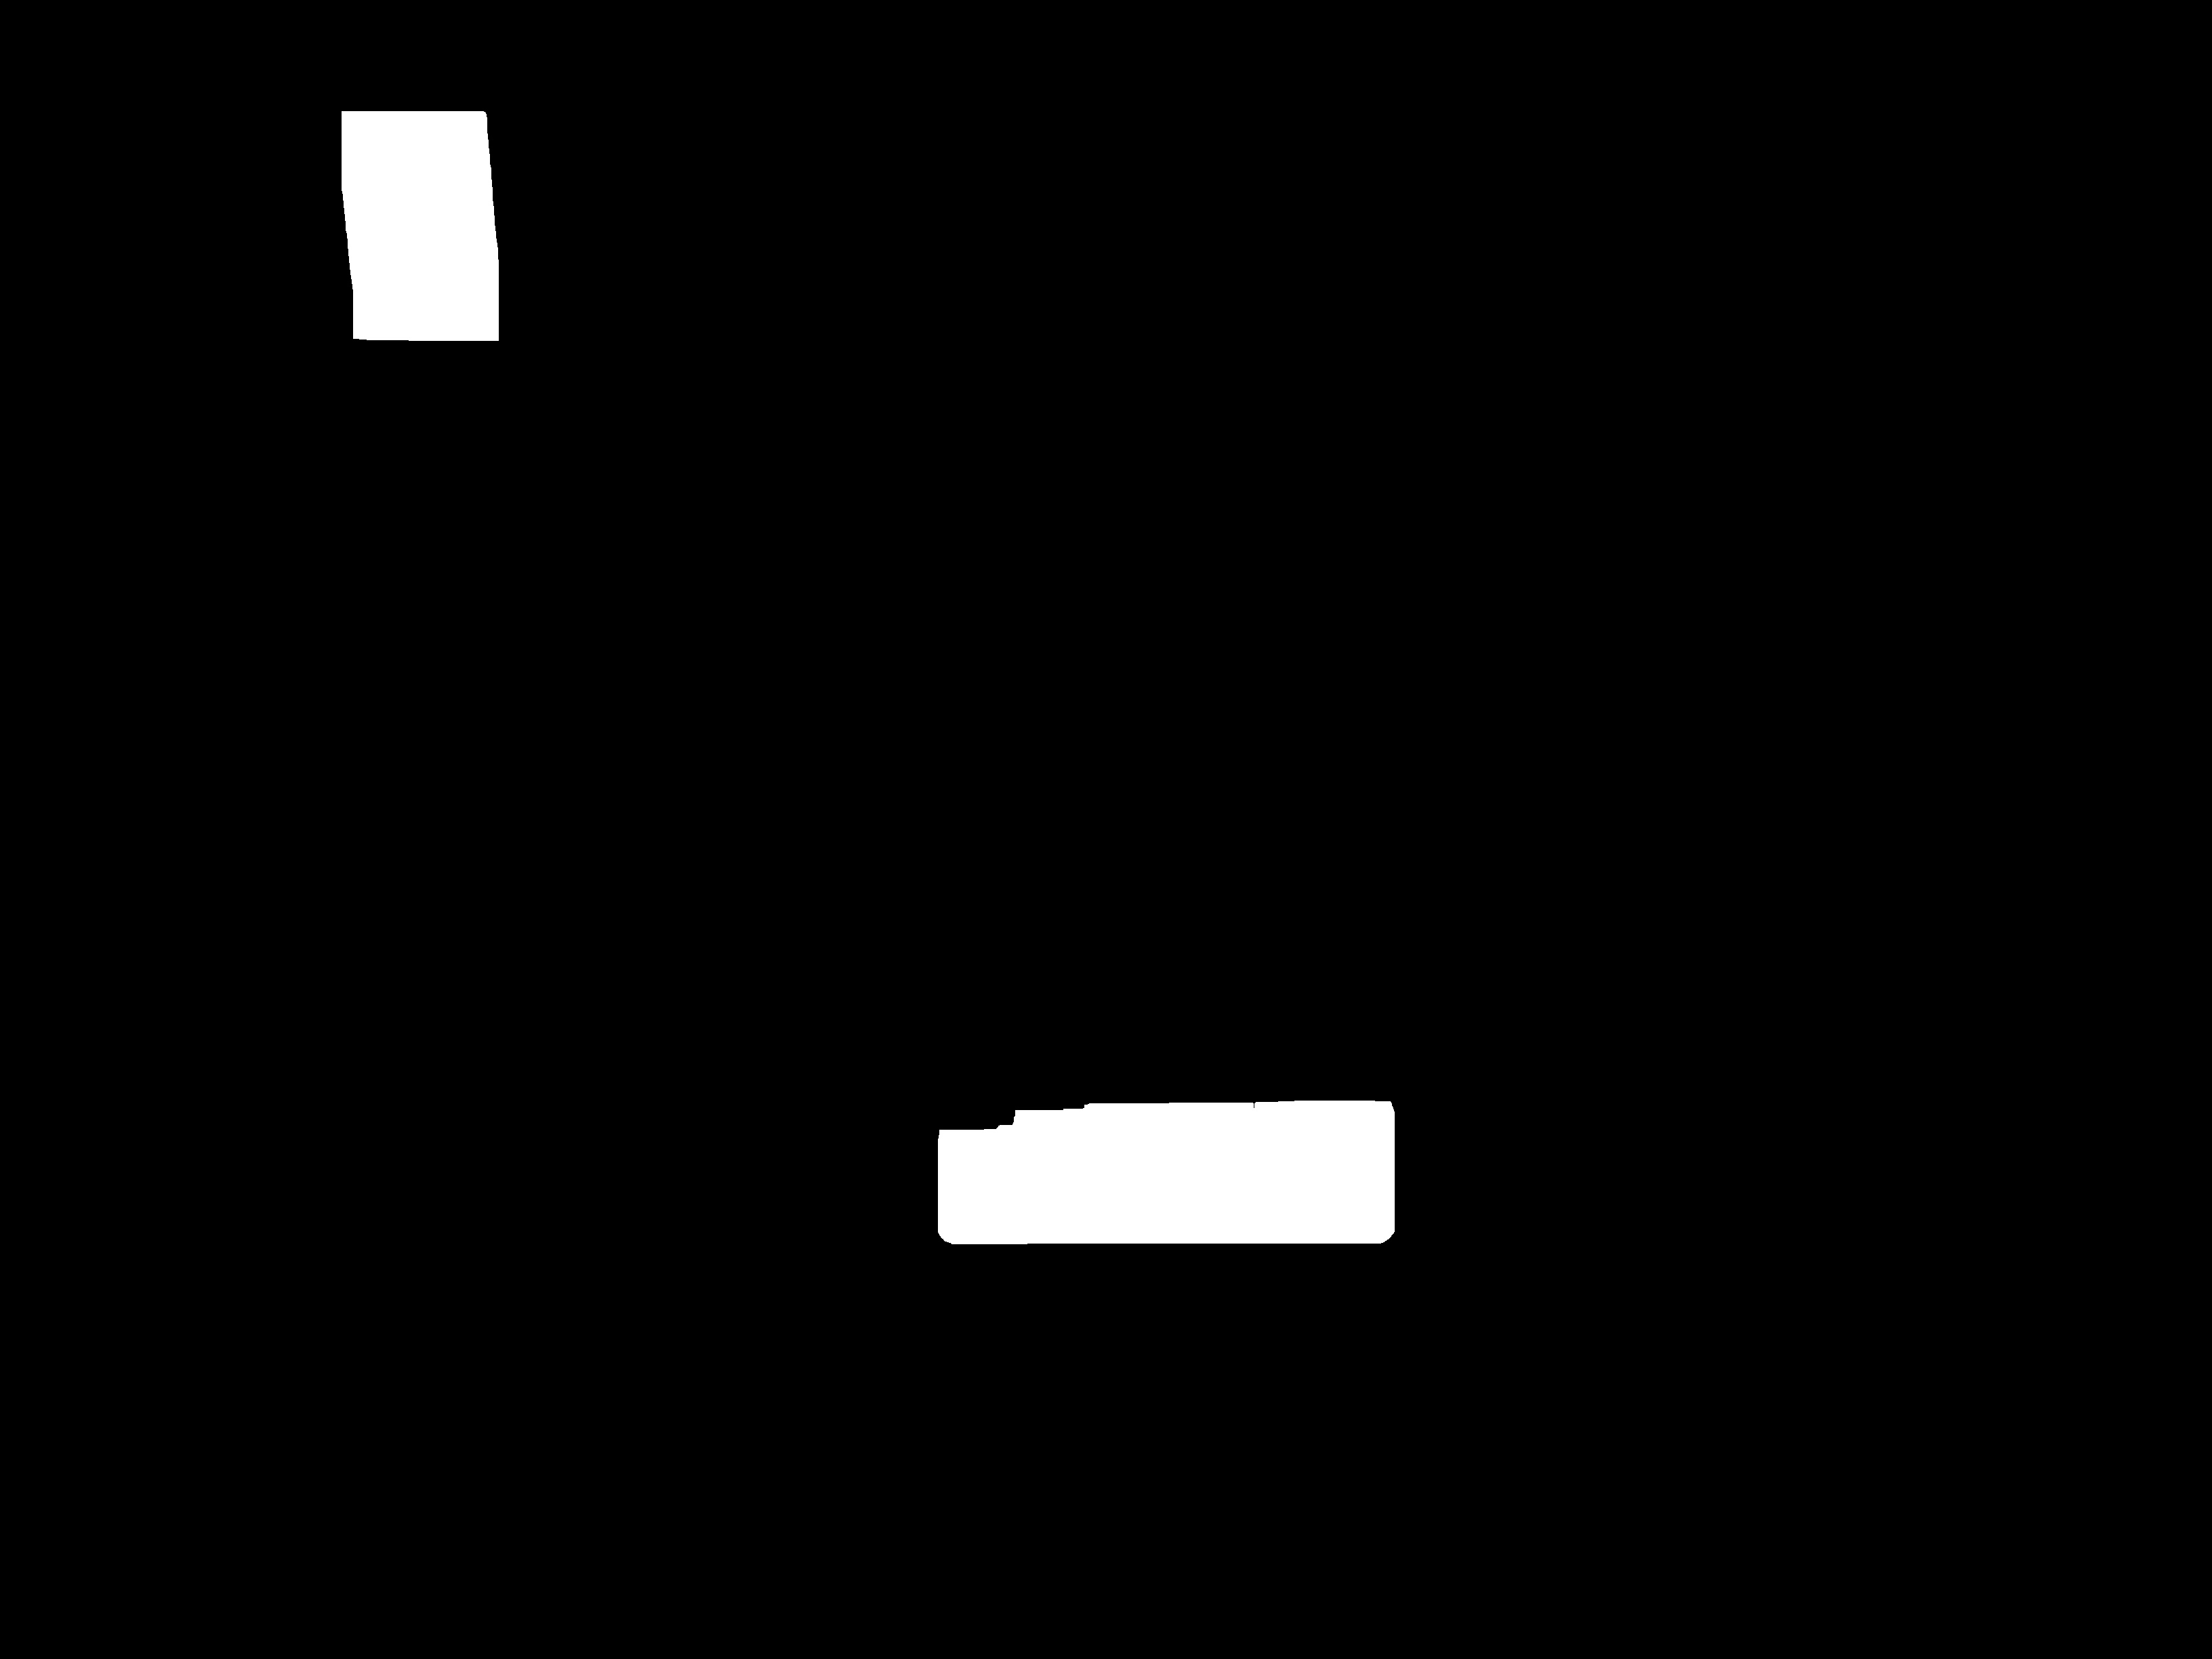
\includegraphics[width=88mm]{9fill_dilated.jpg}
	\caption{Detecção das áreas candidatas da placa}
Fonte: Imagem processada pelo algoritmo
	\label{fig:ext_plate_area_detection}
\end{figure}

\subsection{Extração da área da placa real}

Ao localizar as regiões candidatas onde pode-se encontrar uma placa, pode-se encontrar também regiões falsas, onde não existe placa. Para excluir estas regiões, Jia \cite{jia2007region} sugere que características sejam extraídas para diferenciar corretamente as regiões de placa por outras. 

Diversas características podem ser utilizadas com este propósito. Elas incluem o tamanho da região, a altura e largura da região, a orientação dos caracteres posteriormente extraídos, a intensidade das bordas e a posição da região.
 
Após a detecção da área da placa, essa área é extraída da imagem. Em primeiro lugar, os índices de linha e coluna da área da placa são encontrados por análise de componentes conectados.

\begin{figure}[H]
	\centering
	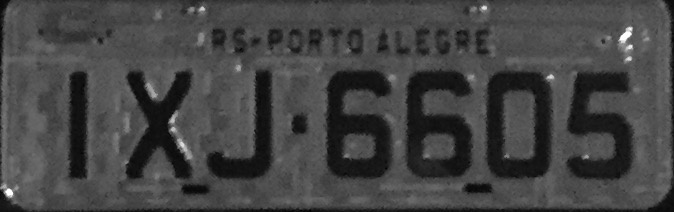
\includegraphics[width=88mm]{a01grayscale.jpg}
	\caption{Placa extraída}
Fonte: Imagem processada pelo algoritmo
	\label{fig:ext_true_number_plate}
\end{figure}

\subsection{Aprimoramento da região extraída}

A placa extraída deve ser convertida para um formato que seja processável pelo algoritmo. É aplicada sobre a imagem a conversão para tons de cinza seguida pela binarização. Apesar de a placa binarizada conter bastante ruídos não são feitas mais operações sobre a imagem da placa. O método seguinte, de segmentação de caracteres, sessão \ref{sec:segmentacao} vai lidar com os ruídos. O motivo da não utilização de algoritmos de remoção de ruído é para não deformar os caracteres a serem lidos pelo reconhecedor de caracteres na sessão \ref{sec:reconhecimento}.

\begin{figure}[H]
	\centering
	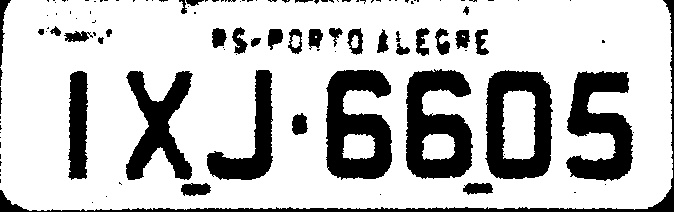
\includegraphics[width=88mm]{a02fill_binary.jpg}
	\caption{Placa aprimorada}
Fonte: Imagem processada pelo algoritmo
	\label{fig:ext_enhanced_number_plate}
\end{figure}

\section{Segmentação dos caracteres}
\label{sec:segmentacao}

O terceiro passo para o reconhecimento da placa é a segmentação dos caracteres.
A segmentação dos caracteres consiste na extração dos caracteres utilizando
estratégias como projetar as suas informações de cores, rotulá-los ou comparar
suas posições com modelos. A placa extraída no passo anterior pode conter
problemas de inclinação ou iluminação, mas o algoritmo de segmentação deve
superar todos esses problemas com pré-processamento.~\cite{s2013automatic}

S Du et al.~\cite{s2013automatic} faz uma análise dos algoritmos de segmentação mais
utilizados com seus prós e contras.  Os principais algoritmos utilizados são:
segmentação utilizando conectividade de \emph{pixels}, segmentação utilizando
perfis de projeção, segmentação utilizando conhecimento anterior dos caracteres,
segmentação utilizando contorno dos caracteres e segmentação utilizando
características combinadas.

O método utilizado une a segmentação utilizando a conectividade de \emph{pixels} com algum conhecimento anterior dos caracteres. É utilizada uma detecção de \emph{pixels} conectados para detectar quais elementos são possíveis caracteres e utilizado o conhecimento sobre a placa para descartar pontos muito pequenos ou muito próximos as bordas da placa.

\begin{figure}[H]
	\centering
	
\includegraphics[width=100mm]{b10filled_characters.png}
	\caption{Preenchimento dos caracteres}
Fonte: Imagem processada pelo algoritmo
	\label{fig:preenchimento}
\end{figure}

O primeiro passo é o preenchimento dos espaços em branco da placa previamente tratada. Este passo existe para evitar que, ao detectar os contornos dos caracteres por meio da conexão dos \emph{pixels}, não aconteça uma dupla detecção em caracteres que contém espaços internos abertos. Por exemplo o número 0, que possui um contorno interno e um contorno externo. Na imagem \ref{fig:preenchimento} podemos ver a placa com os caracteres preenchidos por este passo.

Neste ponto são detectados os contornos com base na conexão dos \emph{pixels}. Muitos \emph{pixels} conectados não fazem parte de nenhum caractere da placa. Para descartar os \emph{pixels} indesejados é feito um filtro baseado no tamanho dos contornos e na sua posição. A altura dos contornos não pode ser menor do que metade da altura da imagem completa. Isso descarta os conjuntos pequenos de \emph{pixels} indesejados. Outro critério é que o contorno encontrado não pode estar encostado na borda da imagem. Em uma placa corretamente extraída os caracteres nunca vão estar encostando na borda. Este critério exclui sombras ou áreas que sobram na lateral da placa na extração, que poderiam ser erroneamente confundidas com caracteres.

\begin{figure}[H]
	\centering
	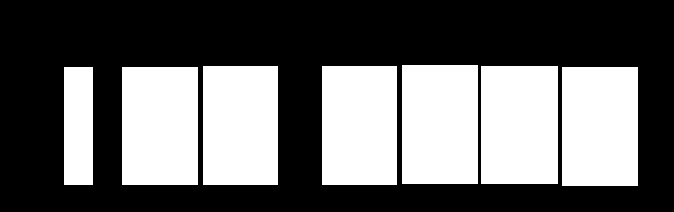
\includegraphics[width=100mm]{b20mask.png}
	\caption{Máscara gerada}
Fonte: Imagem processada pelo algoritmo
	\label{fig:mascara}
\end{figure}

Encontrados os contornos dos caracteres corretos, uma máscara, mostrada na figura\ref{fig:mascara}, é feita a partir deles que será aplicada sobre a imagem da placa extraída original. Esta máscara irá desconsiderar tudo, apenas o conteúdo extraído na etapa anterior. Os caracteres recortados com base nesta máscara serão extraídos, ordenados com base em sua posição x, e enviados para a etapa de reconhecimento de caracteres.

\begin{figure}[H]
	\centering
	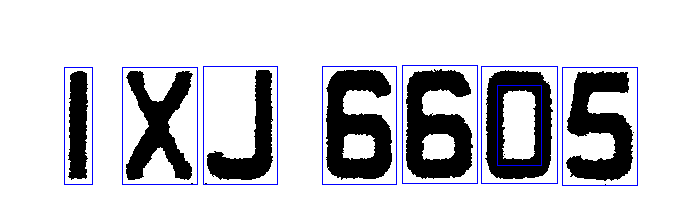
\includegraphics[width=100mm]{a08character_borders.png}
	\caption{Caracteres a serem extraídos}
Fonte: Imagem processada pelo algoritmo
	\label{fig:caracteres_extraidos}
\end{figure}

\section{Reconhecimento dos caracteres} \label{sec:reconhecimento}

O último passo para reconhecimento da placa é o reconhecimento ótico dos
caracteres extraídos. Um dos maiores desafios da extração de caracteres é o fato de
os caracteres extraídos não terem o mesmo tamanho e grossura, devido ao
\emph{zoom} da câmera. Outro problema, ao criar um reconhecedor de propósito
geral, é as diferentes fontes das diferentes placas ao redor do mundo.~\cite{s2013automatic}
Este segundo não será um problema para este trabalho pois
só há interesse em reconhecer placas brasileiras. Outro desafio é o
reconhecimento de caracteres semelhantes, como o D e o
0~\cite{ho2016intelligent}.  Esse problema será mitigado com o conhecimento
prévio das placas brasileiras, sabendo onde é possível haver letras e onde é
possível haver números.

Tendo em mente os possíveis problemas foi implementado um reconhecedor de caracteres especificamente para a solução deste problema. Foi utilizado o algoritmo \emph{K-Nearest Neighbors} para classificar os caracteres possíveis e utilizados os caracteres na fonte \emph{Mandatory} dispostos na imagem~\ref{fig:tipografia} como dados de treinamento. O \emph{feature space} consiste de um caractere apenas por classe, portanto será utilizado apenas um vizinho para classificar o novo dado.

Além de focar na fonte na qual as placas estão escritas, o reconhecedor é calibrado também para o padrão. Sabendo que a placa de transito tem três letras e quatro números, mantendo esta ordem, o reconhecedor nunca vai confundir uma letra com um número. Para conseguir este resultado utilizamos dois diferentes \emph{feature spaces}, um para os números e um para as letras. Assim, quando classificamos um caractere novo, ele será classificado somente entre os possíveis candidatos.

Para que a classificação tenha sucesso, tanto as imagens de teste quanto as imagens a serem classificadas devem ter o mesmo tamanho. O \emph{feature space} deve ter \emph{N} dimensões não variáveis. Para isso as imagens são tratadas para que tenham todas o tamanho de 100x100 \emph{pixels}, preenchendo o espaço restante com \emph{pixels} brancos

\begin{figure}[H]
	\centering
	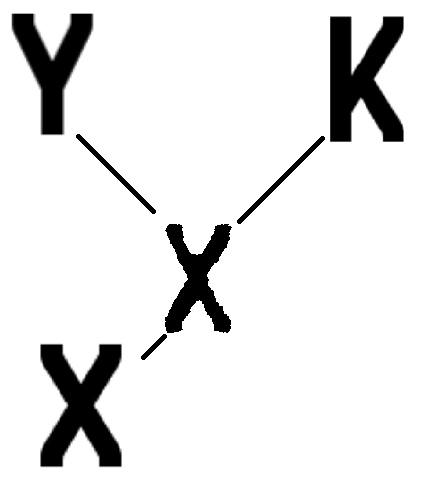
\includegraphics[width=50mm]{classificacao.png}
	\caption{Exemplo de classificação de caractere extraído}
Fonte: Imagens utilizadas como dados de treino e imagem processada pelo algoritmo
	\label{fig:classificacao}
\end{figure}

Na figura \ref{fig:classificacao} são mostrados os três vizinhos mais próximos de um determinado caractere retirado do processamento de uma imagem. A sua projeção visual é hipotética e foi criada para representar de uma forma mais didática a seleção dos vizinhos. Pode-se reparar a semelhança entre os caracteres e entender porque eles foram selecionados ao visualizar a imagem.